% Midterm Report -- AI Agents for Kaggle Competitions
% Compile with pdfLaTeX (Overleaf default). No external assets required.
\documentclass[11pt,a4paper]{article}

\usepackage[margin=2.5cm]{geometry}
\usepackage{amsmath,amssymb}
\usepackage{newtxtext,newtxmath}
\usepackage{float}
\usepackage[section]{placeins}
\usepackage{booktabs}
\usepackage{caption}
\usepackage{microtype}
\usepackage{array}
\usepackage{enumitem}
\usepackage[hyphens]{url}
\usepackage[colorlinks=true, linkcolor=black, citecolor=black, urlcolor=blue!50!black]{hyperref}
\usepackage{xcolor}
\usepackage{tikz}
\usetikzlibrary{positioning,arrows.meta,calc,decorations.pathreplacing}

\emergencystretch=1.5em

\captionsetup{font=small,labelfont=bf}
\newcolumntype{L}[1]{>{\raggedright\arraybackslash}p{#1}}
\renewcommand{\arraystretch}{1.15}
\newcommand{\TBD}[1]{\textcolor{orange!85!black}{\textbf{[TBD: #1]}}}
\newcommand{\dn}{\ensuremath{\downarrow}}
\newcommand{\up}{\ensuremath{\uparrow}}
% Agent abbreviations used in verdict columns
\newcommand{\M}{M}   % my-agent
\newcommand{\N}{N}   % NVIDIA
\newcommand{\A}{A}   % AIDE

\title{\textbf{Benchmarking AI Agents for Kaggle Competitions:\\
A Fair Three-Way Comparison with Paired Significance Testing}\\
\large Report v3 --- CONDENSED DRAFT (August 2026)\\
\normalsize\textcolor{orange!85!black}{All printed numbers are real measurements as of 2026-07-30; pending results are marked [TBD].}}
\author{Wei-Hao Huang\\\small Advisor: Tso-Jung Yen}
\date{Draft compiled July 30, 2026}

\begin{document}
\maketitle

\begin{center}\textbf{\large Abstract}\end{center}
\noindent LLM-driven coding agents can now solve machine-learning competitions end-to-end, but evaluating them has not kept pace: comparisons typically report one run and one score per competition, ignoring both test-set sampling error and the stochasticity of agent execution. We benchmark three methodologically distinct agents --- \textbf{my-agent}, our hybrid of LLM reasoning, Auto-ML tools, and a cross-competition experience library; \textbf{AIDE}, LLM tree search with no cross-competition memory; and the \textbf{NVIDIA Kaggle Agent}, which reproduces the highest-voted public kernel --- on 18 tabular Kaggle competitions under a mechanically enforced fairness protocol, scoring every submission on the real leaderboard, and extend the comparison to three mid-complexity competitions spanning NLP, physiological time series, and medical imaging, where my-agent takes the three-way best on all three under equal budgets and a cold experience base. We introduce a paired significance test whose error scale comes free from Kaggle's public/private test split: a win counts only if the ordering replicates across the two disjoint subsets and the gap exceeds its own movement. Under this test my-agent wins 59\% of decidable duels versus 46\% (AIDE) and 45\% (NVIDIA), while 26\% of duels are statistically undecidable. Local cross-validation disagrees with the true leaderboard in 10 of the 13 competitions where both are available, and the three-way ranking fully reverses when the composition of the evaluation set changes. Guided by the failure-mode analysis, we then move knowledge injection from the post-hoc blend stage (measured gain ${\sim}10^{-5}$) to the \emph{problem-identification stage}: a dossier layer that classifies each task and decides split policy and external-data need before any modeling. Across all 18 competitions the layer achieves perfect separation (fires on exactly the 2 country-panel time-series tasks; zero false positives on the other 16), and on s3e19 --- the benchmark's canonical failure --- it significantly beats the frozen v3 baseline under the same paired leaderboard test (private SMAPE 48.24 vs.\ 50.46), lifting my-agent from clearly last on that competition to numerically first among the three. A controlled follow-up on s3e19 and a held-out replication competition finds that all four external-data arms beat their no-external baselines significantly, but that neither cross-validation nor a held-out-year protocol can choose which \emph{form} the injection should take --- local signals rank the forms wrongly, and in opposite directions on the two competitions. Leaderboard probes further decompose s3e19's residual into ${\sim}15.5$ points of level error and ${\sim}33$ of shape, showing that the external join is worth only $6.0$ of a 44-point gap and correcting the explanation our own midterm gave for this failure. Agent-benchmark claims must be stated jointly with an error model and the composition of the evaluation set; knowledge injection pays where problems are identified rather than where predictions are blended; and a judgment layer must be reported together with what consumes its proposals, not only with how many it can express: of 241 proposals 73\% are expressible, but tracing the consumers found only 5\% applied by the code reporting them, 32\% emitted to a reader that did not exist, and 14\% owned by another layer --- a produced-but-unconsumed artifact reads exactly like a success.

\vspace{0.5em}

\section{Introduction}

Machine-learning competitions are \emph{scorable tasks}: a submission receives a single measurable quality score on a hidden test set, and a public leaderboard records how it compares against thousands of human teams. Solving them end-to-end --- data understanding, validation design, feature engineering, model selection, ensembling --- has traditionally demanded expert labor and extensive trial and error. LLM-driven coding agents have recently begun to automate this loop: AIDE performs LLM-guided tree search over candidate solutions~\cite{aide2025}; ERA couples an LLM rewriter with tree search and externally injected research ideas, outperforming strong baselines across 16 Kaggle Playground competitions~\cite{aygun2026}; and industrial agents skip search altogether by reproducing the strongest public solution to a given competition~\cite{nvidia2026}.

However, \emph{evaluating competition agents is currently far less rigorous than building them}. Comparisons typically report one run and one score per competition and declare the higher number the winner. Two error sources make this fragile. Competition metrics carry test-set sampling error, and top-two gaps often sit at the fourth or fifth decimal place. Agent execution is itself stochastic --- the LLM samples different code at every step. When the gap between two agents is smaller than these errors, ``A beats B'' is reporting noise. Nor does self-evaluation offer an escape: without external, methodologically different reference points, any assessment of one's own agent is circular.

Here we present a controlled three-way benchmark of methodologically distinct agents: \textbf{my-agent}, our hybrid design combining LLM reasoning, Auto-ML tools, and a cross-competition experience library (Figures~\ref{fig:arch} and \ref{fig:tree}); \textbf{AIDE}, LLM tree search with no cross-competition memory; and the \textbf{NVIDIA Kaggle Agent}, which reproduces the highest-voted public kernel. Both reference methods are frozen for the duration of the study. All three agents run on 18 Kaggle competitions under a mechanically enforced fairness protocol (Section~\ref{sec:fairness}), and every submission is scored on the real leaderboard via late submission. Critically, each competition scores one submission on two disjoint test subsets --- public and private --- and we turn this split into a paired significance test: a win counts only if the ordering replicates across both subsets and the gap exceeds its own movement (Section~\ref{sec:exp2}).

Guided by what the benchmark revealed, we then act on it. The failure-mode analysis identifies problem-level judgment --- ``does this task need external data?'', ``is the test set a future time window?'' --- as the shared gap of all three agents, and our own measurement shows that injecting knowledge post hoc at the blend stage is worth only ${\sim}10^{-5}$. We therefore introduce a \emph{problem-identification layer} (v5): a dossier stage that runs before EDA, matches each competition against an evidence-backed library of task-level priors, and drives a whitelisted, leakage-guarded external-data module (Section~\ref{sec:v5}). The layer is evaluated the same way the agents are --- swept across all 18 competitions for specificity and sensitivity, then subjected to a controlled causal test on the benchmark's canonical failure plus a held-out replication competition, and finally audited for how much of what it proposes the execution layer can actually run (Sections~\ref{sec:exp5v5} and~\ref{sec:exp6v5}).

We find that my-agent wins 59\% of decidable duels versus 46\% (AIDE) and 45\% (NVIDIA), while 26\% of duels are statistically undecidable --- verdicts that a naive tally would have reported as conclusions. We further find that local cross-validation disagrees with the true leaderboard in 10 of the 13 competitions where both are available, and that the three-way ranking fully reverses when the evaluation set shifts from Playground-only to a broader mix. A ranking is a property of the method \emph{and} the evaluation set; benchmark claims must be stated jointly with both. The same discipline applied to our own new layer yields one clear positive and one clear negative: external-data injection beats its matched baseline in all four controlled arms we ran, and no local validation protocol we tried can select the form that injection should take.

\section{Methods}

\subsection{my-agent: A Hybrid Kaggle Agent}

The method is implemented as a Claude Code Skill (\texttt{kaggle-agent}). Its core design is a division of labor between LLM reasoning and Auto-ML tools: the LLM (Claude Code) handles problem understanding, validation-strategy design, creative feature engineering, result interpretation, and deciding the next step; LightGBM / XGBoost / CatBoost / Optuna --- invoked by the LLM via the shell --- handle model selection, hyperparameter optimization, and stacking/ensembling.

Execution proceeds in six stages: data ingestion $\to$ EDA $\to$ feature engineering $\to$ modeling $\to$ evaluation $\to$ submission, where stages four and five run in one of two optimization modes:

\begin{itemize}[leftmargin=*]
  \item \textbf{Linear iteration protocol}: propose a hypothesis, run the experiment, record the result --- used for the first pass and for small competitions.
  \item \textbf{Tree search (preferred)}: once the linear protocol has produced a baseline single model and at least one blend, the agent switches to tree search (harness v3; protocol in Figure~\ref{fig:tree}). Internal evaluation shows tree search winning 9 of 10 competitions with 1 tie and 0 losses.
\end{itemize}

Two supporting mechanisms:

\paragraph{Cross-competition experience library} (\path{knowledge/experience.md}): every insight must carry an evidence field (\texttt{competition, exp \#N, score A $\to$ score B}); entries without a score delta are rejected. The agent queries the library before EDA and before modeling, and writes validated new insights back after experiments. This is the most fundamental design difference between my-agent and the two reference methods.

\paragraph{Experiment records.} Every experiment's parameters, features, split scheme, and scores are logged in structured form (\path{experiments.json}, \path{experiments_tree_v3.json}), making every number in this report traceable.

Figure~\ref{fig:arch} summarizes the architecture and how the two mechanisms connect to the search loop.

\begin{figure}[htbp]
\centering
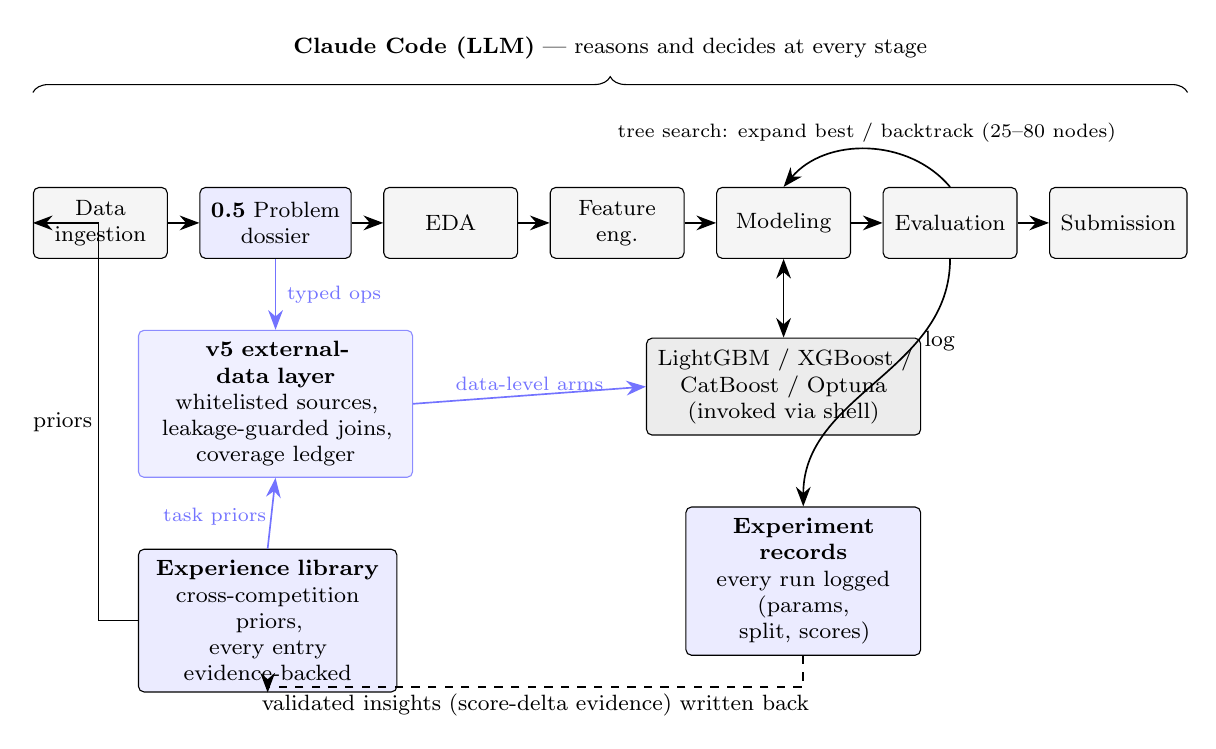
\begin{tikzpicture}[
  font=\footnotesize,
  stage/.style={draw, rounded corners=2pt, align=center, inner sep=4pt, fill=gray!8, minimum height=9mm, minimum width=17mm},
  mech/.style={draw, rounded corners=2pt, align=center, inner sep=4pt, fill=blue!8},
  tool/.style={draw, rounded corners=2pt, align=center, inner sep=4pt, fill=gray!15},
  arr/.style={-{Stealth[length=2.5mm]}, semithick},
  darr/.style={arr, dashed}
]
% pipeline: Stage 0.5 sits before EDA
\node[stage] (s1) {Data\\ingestion};
\node[stage, right=4mm of s1, fill=blue!8] (s05) {\textbf{0.5} Problem\\dossier};
\node[stage, right=4mm of s05] (s2) {EDA};
\node[stage, right=4mm of s2] (s3) {Feature\\eng.};
\node[stage, right=4mm of s3] (s4) {Modeling};
\node[stage, right=4mm of s4] (s5) {Evaluation};
\node[stage, right=4mm of s5] (s6) {Submission};
\foreach \a/\b in {s1/s05, s05/s2, s2/s3, s3/s4, s4/s5, s5/s6}{\draw[arr] (\a) -- (\b);}
% LLM annotation above
\draw[decorate, decoration={brace, amplitude=2mm}]
  ([yshift=12mm]s1.north west) -- ([yshift=12mm]s6.north east)
  node[midway, above=3mm]{\textbf{Claude Code (LLM)} --- reasons and decides at every stage};
% tree-search loop over stages 4-5
\draw[arr] (s5.north) to[out=130, in=50]
  node[pos=0.5, above=0.5mm, inner sep=1pt]{\scriptsize tree search: expand best / backtrack (25--80 nodes)} (s4.north);
% auto-ml tools under modeling
\node[tool, below=10mm of s4, text width=32mm] (tools)
  {LightGBM / XGBoost /\\CatBoost / Optuna\\(invoked via shell)};
\draw[arr, {Stealth[length=2.5mm]}-{Stealth[length=2.5mm]}] (s4.south) -- (tools.north);
% --- row 2: v5 execution layer (under the dossier) and Auto-ML tools (under modeling) ---
\node[tool, below=9mm of s05, text width=32mm, fill=blue!6, draw=blue!45] (ext)
  {\textbf{v5 external-data layer}\\whitelisted sources,\\leakage-guarded joins,\\coverage ledger};
\draw[arr, blue!55] (s05.south) -- node[right=1mm, inner sep=1pt, pos=0.5]{\scriptsize typed ops} (ext.north);
\draw[arr, blue!55] (ext.east) -- node[above, inner sep=1.5pt, pos=0.5]{\scriptsize data-level arms} (tools.west);
% --- row 3: the two cross-cutting mechanisms, clear of row 2 ---
\node[mech, below=9mm of ext.south west, text width=30mm, anchor=north west] (lib)
  {\textbf{Experience library}\\cross-competition priors,\\every entry evidence-backed};
\node[mech, below=9mm of tools.south east, text width=27mm, anchor=north east] (rec)
  {\textbf{Experiment records}\\every run logged\\(params, split, scores)};
\draw[arr, blue!55] (lib.north) -- node[left, inner sep=1.5pt, pos=0.45]{\scriptsize task priors} (ext.south);
\draw[arr] (lib.west) -- ++(-5mm,0) |- node[left, inner sep=2pt, pos=0.25]{priors} (s1.west);
\draw[arr] (s5.south) to[out=270, in=90] node[right, inner sep=2pt, pos=0.3]{log} (rec.north);
% write-back loop
\draw[darr] (rec.south) -- ++(0,-4mm) -| node[near start, below, inner sep=2pt]{validated insights (score-delta evidence) written back} (lib.south);
\end{tikzpicture}
\caption{Architecture of my-agent. The LLM drives every stage; modeling and evaluation iterate
via tree search and invoke Auto-ML tools through the shell, while two cross-cutting mechanisms
close the loop --- the experience library supplies evidence-backed priors, and every run is
logged, with score-delta-validated insights written back. Shown in blue is v5, the upstream
layer this report adds: \textbf{Stage 0.5} runs \emph{before} EDA and decides what kind of
problem this is --- task family, train--test window relation, split policy, external-data need
--- emitting typed operators from a closed vocabulary. Those drive a whitelisted,
leakage-guarded external-data layer whose data-level arms are raced against the no-external
baseline. The placement is the claim: the same knowledge injected downstream at the blend stage
measured ${\sim}10^{-5}$ (Section~\ref{sec:v5}).}
\label{fig:arch}
\end{figure}

\paragraph{Tree-search protocol.} Every run in this report uses harness v3: a node is a
complete solution, ensembles are first-class node kinds with out-of-fold caching and weight
search, and a budget phase machine exploits until all lineages plateau, then forces one
exploration burst, then stops. Figure~\ref{fig:tree} shows the loop. A later v4 adds external
idea injection at the blend stage; no benchmark submission here used it, and measuring it
separately on 15 competitions is what motivated moving injection upstream instead --- reweighting
the existing pool never displaced the champion blend (8/8), and expanding the pool improved it in
2 of 8 rigorously measurable competitions, both by ${\sim}10^{-5}$ (Section~\ref{sec:v5}).

\begin{figure}[htbp]
\centering
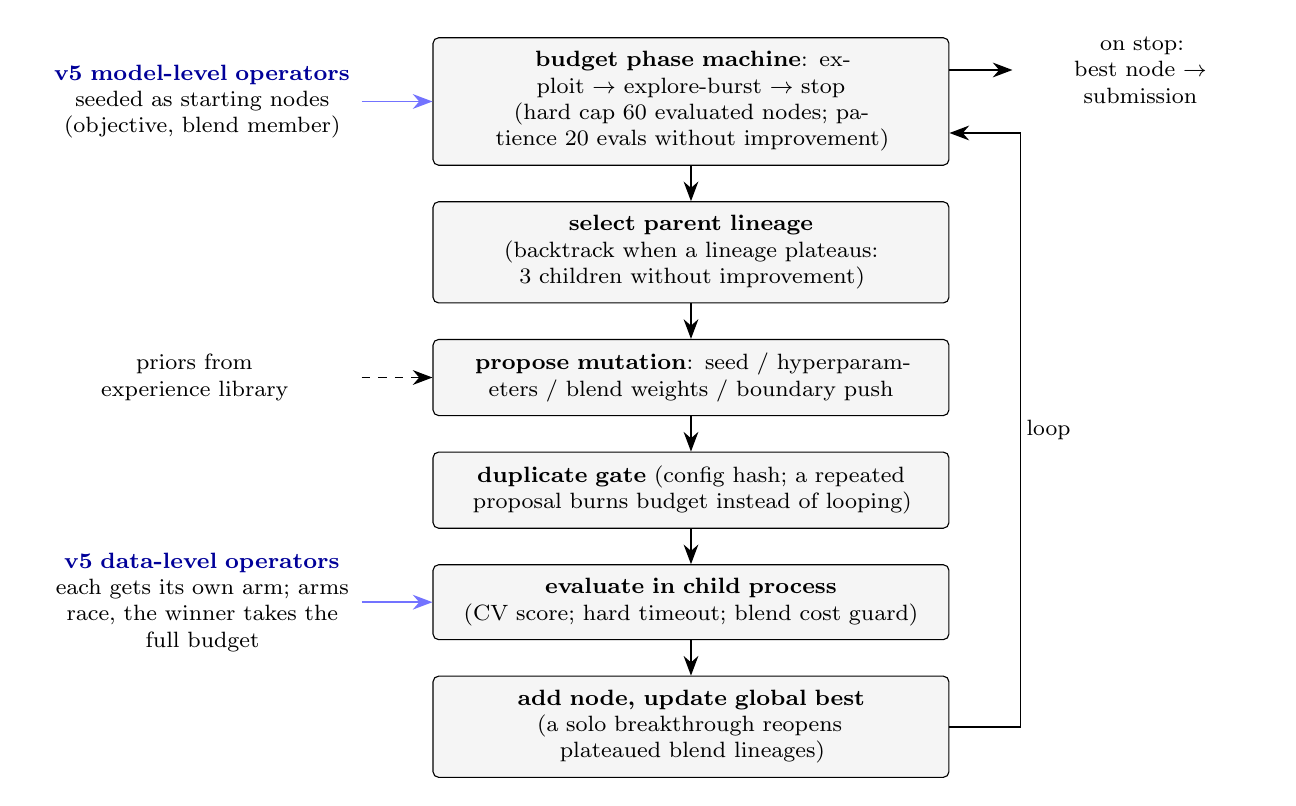
\begin{tikzpicture}[
  font=\footnotesize,
  sbox/.style={draw, rounded corners=2pt, align=center, inner sep=5pt, fill=gray!8, text width=62mm},
  side/.style={align=center, text width=40mm},
  arr/.style={-{Stealth[length=2.5mm]}, semithick},
  node distance=4.5mm
]
\node[sbox] (phase) {\textbf{budget phase machine}: exploit $\to$ explore-burst $\to$ stop\\(hard cap 60 evaluated nodes; patience 20 evals without improvement)};
\node[sbox, below=of phase] (select) {\textbf{select parent lineage}\\(backtrack when a lineage plateaus: 3 children without improvement)};
\node[sbox, below=of select] (propose) {\textbf{propose mutation}: seed / hyperparameters / blend weights / boundary push};
\node[sbox, below=of propose] (dedup) {\textbf{duplicate gate} (config hash; a repeated proposal burns budget instead of looping)};
\node[sbox, below=of dedup] (eval) {\textbf{evaluate in child process}\\(CV score; hard timeout; blend cost guard)};
\node[sbox, below=of eval] (add) {\textbf{add node, update global best}\\(a solo breakthrough reopens plateaued blend lineages)};
\foreach \a/\b in {phase/select, select/propose, propose/dedup, dedup/eval, eval/add}{\draw[arr] (\a) -- (\b);}
% loop back
\draw[arr] (add.east) -- ++(9mm,0) |- node[pos=0.25, right, inner sep=2pt]{loop} ([yshift=-4mm]phase.east);
% priors in
\node[side, left=9mm of propose] (prior) {priors from\\experience library};
\draw[arr, dashed] (prior) -- (propose);
% v5 entry points: seeded nodes and a whole raced lane
\node[side, left=9mm of phase, text width=38mm, align=center] (v5cfg)
  {\textcolor{blue!60!black}{\textbf{v5 model-level operators}}\\seeded as starting nodes\\(objective, blend member)};
\draw[arr, blue!55] (v5cfg) -- (phase);
\node[side, left=9mm of eval, text width=38mm, align=center] (v5data)
  {\textcolor{blue!60!black}{\textbf{v5 data-level operators}}\\each gets its own arm; arms\\race, the winner takes the\\full budget};
\draw[arr, blue!55] (v5data) -- (eval);
% exit
\node[side, right=8mm of phase, yshift=4mm, text width=30mm] (out) {on stop:\\best node $\to$ submission};
\draw[arr] ([yshift=4mm]phase.east) -- (out.west);
\end{tikzpicture}
\caption{The v3 tree-search loop used in all my-agent runs of this report (25--80 nodes per
competition). Each node is a complete, executable solution scored by local cross-validation;
lineages are abandoned on plateau and the budget phase machine forces an exploration burst
before stopping. In blue, where v5's typed operators enter: model-level ones
(\texttt{objective}, \texttt{blend\_member}) are translated into seed nodes the search starts
from, while data-level ones (the external joins) each build their own arm --- a separate
workspace with its own feature table --- and the arms race at small budget before the winner
receives the full one. The distinction matters because it is what makes the arm comparison
controlled: arms differ only by the operator's added columns, everything else digit-identical.}
\label{fig:tree}
\end{figure}

\subsection{v5: Upstream Knowledge Injection}
\label{sec:v5}

The v4 harness injected external ideas at the blend stage and measured a negligible effect (reweighting never displaced the convex-optimum champion in 8/8 rigorous competitions; pool expansion helped 2/8 by ${\sim}10^{-5}$). v5 moves the injection point upstream, where the failure-mode analysis (Section~\ref{sec:exp4}) locates the actual gap:

\paragraph{Stage 0.5 --- problem dossier.} Before EDA, the agent answers ``what kind of problem is this?'': task family, train--test window relation, split policy, and external-data need, written to a structured \path{dossier.json}. Judgments are grounded in \path{knowledge/task_priors.md}, a library of task-level priors each carrying an evidence field from our own benchmark (e.g., the shuffled-KFold $4.5\times$ bias; the GDP-join CV gap on jan-2022). Reading competition-specific discussions or kernels is forbidden --- the dossier must derive from the problem statement plus task-\emph{type} knowledge only, keeping the method distinct from reproduction-based agents. The dossier is a prior, not a conclusion: EDA must verify its hypotheses and record a verdict.

\paragraph{External-data module.} A whitelist of public sources (eight World Bank indicators, ECB monthly FX, OWID COVID, holiday calendars, ISO tables), each fetched with recorded snapshots and joined through leakage-guarded as-of merges: an external value may reach a prediction row only if dated at or before the row's period minus a declared lag; violations raise; numeric time columns must declare their unit; every join writes an audit log. The module was adversarially verified (21 reproduced findings, including three silent-future-leak classes, all fixed with regression tests).

\paragraph{Search integration.} Data-level dossier ideas spawn their own variant workspaces raced at small tree-search budget (an idea that changes the data gets its own lane); model-level ideas enter the main tree as seed lineages. The winning lane receives the full search budget.

\paragraph{A typed contract between the two layers.} The first version of this stack failed
instructively: the dossier correctly proposed World Bank GDP for s3e19 \emph{as a country-level
scale covariate}, and the experience library already held the operational recipe, but the
execution layer could express exactly one transformation --- appending a column to the feature
list. Since a gradient-boosted tree cannot extrapolate a feature beyond its training range, the
semantics of ``scale covariate'' evaporated between the layers with nothing raising an error.
The fix is a closed vocabulary both layers read (\path{knowledge/injection_operators.md}): ten
typed operators, each with a parameter schema, the evidence justifying it, and explicit
conditions under which it must \emph{not} be used. The dossier may emit only these, each
carrying its rationale and source prior; anything the vocabulary cannot express is written to
\texttt{not\_recorded} rather than into prose the execution layer will ignore. The dispatcher
writes a coverage ledger --- proposed, realized, unrealized-with-reason --- so an unimplemented
capability leaves a trace instead of resembling success. Two automatic preconditions guard the
level-covariate operators: proportionality and covariate volatility. Conformance is
machine-checked on both sides (Appendix~\ref{app:coverage}).

\subsection{Two Reference Methods (Yardsticks)}

\paragraph{AIDE} (open-source agent, gen-1): LLM-driven tree search. At each step it writes a complete solution, executes it, reads the error or score, and mutates accordingly. No cross-competition memory --- every competition starts from zero; the journal only persists within a single run. Executed with its default budget of 20 steps.

\paragraph{NVIDIA Kaggle Agent} (skill): its method is ``reproduce the strongest public kernel'' --- research the competition context, select the highest-\emph{voted} solution-type kernel, port it faithfully, and retrain on local data. Its knowledge comes from publicly available solutions fetched fresh each time; nothing accumulates across competitions.

\paragraph{Key methodological decision.} Both reference methods are frozen --- no improvements of any kind. During the study we found that NVIDIA's vote-based kernel selection is a structural weakness (Section~\ref{sec:exp4}), and the skill itself even ships a score-based selection tool, but we deliberately did not enable it. Rationale: the purpose of this study is to use them as fixed yardsticks for measuring my-agent; improving the yardsticks mid-study would make earlier and later data incomparable, and would quietly turn the benchmark into an optimization of the reference methods.

\subsection{Fairness Protocol}
\label{sec:fairness}

The three agents share one machine, so the rules in Table~\ref{tab:fairness} are defined and mechanically enforced.

\begin{table}[htbp]
\centering\small
\caption{Fairness protocol: rules and their enforcement.}
\label{tab:fairness}
\begin{tabular}{@{}L{2.4cm}L{6.6cm}L{5.6cm}@{}}
\toprule
\textbf{Aspect} & \textbf{Rule} & \textbf{Enforcement} \\
\midrule
Data isolation & Each side reads only \path{bench-comps/<comp>/}, containing files validated against the official Kaggle manifest & \path{build_isolated_roots.py}; officialness judged by the Kaggle API manifest, incl.\ members extracted from official archives \\
Workspace isolation & The three output directories are fully separated; each side is scored independently & Directory structure \\
Instruction isolation & Prompts may contain only environment facts and metric thresholds; no modeling recipes, no other side's scores, no environment workarounds discovered by another side & Manual protocol + incident log \\
Resource isolation & Only one lane executes at any moment & \path{lane_lock.sh} mutex (atomic directory creation, reclamation on holder death, bounded waiting) \\
Environment defects & Always fix the environment rather than give hints (fixing removes the confound; hinting compensates only one side) & --- \\
\bottomrule
\end{tabular}
\end{table}

\section{Experiments}

\subsection{Overview of Experimental Design}

\paragraph{Evaluation set.} 18 tabular competitions --- 13 from the Kaggle Playground Series, plus afsis-soil-properties (2014, spectral regression), conway-s-reverse-game-of-life (2014, structured multi-output), cat-in-the-dat (2019, purely categorical features), tabular-playground aug-2022, and jan-2022. Every competition provides both a public and a private test-subset score --- this is the inclusion criterion, because the significance test (Section~\ref{sec:exp2}) is built on the score difference between the two subsets. The three agents also ran 4 competitions for which private scores cannot be obtained (late submission closed, rolling leaderboards); these are excluded. The 18-competition set is the fixed baseline of this study.

\paragraph{Execution conditions.} The three agents ran serially, with the mutex guaranteeing no overlap. AIDE: 20 steps (its default budget; conway stopped at 16 steps due to the 4-hour cap). NVIDIA: reproduced public kernels per its method. my-agent: the full six-stage pipeline including tree search (25--80 nodes per competition; Appendix~\ref{app:treesize}).

\subsection{Experiment 1: Three-Way Capability Comparison (Raw Scores)}
\label{sec:exp1}

\paragraph{Goal and procedure.} Measure the absolute performance of the three methods on the same set of competitions. Each side independently produces a submission, uploaded to Kaggle via late submission to obtain public and private scores, along with the percentile rank relative to all participating teams of that competition.

\begin{table}[htbp]
\centering\small
\caption{Competition descriptions. Tasks fall into two families: classification (binary, ordinal; 7 competitions) and prediction/regression (incl.\ time series and multi-target; 11 competitions).}
\label{tab:comps}
\begin{tabular}{@{}rllr@{}}
\toprule
\# & \textbf{Competition} & \textbf{Task type} & \textbf{Train rows $\times$ cols} \\
\midrule
1 & s3e1 & Regression & $37{,}137 \times 10$ \\
2 & s3e3 & Classification (binary) & $1{,}677 \times 35$ \\
3 & s3e5 & Classification (ordinal) & $2{,}056 \times 13$ \\
4 & s3e7 & Classification (binary) & $42{,}100 \times 19$ \\
5 & s3e9 & Regression & $5{,}407 \times 10$ \\
6 & s3e11 & Regression & $360{,}336 \times 17$ \\
7 & s3e14 & Regression & $15{,}289 \times 18$ \\
8 & s3e16 & Regression & $74{,}051 \times 10$ \\
9 & s3e19 & Regression (time series) & $136{,}950 \times 6$ \\
10 & s4e11 & Classification (binary) & $140{,}700 \times 20$ \\
11 & s5e10 & Regression & $517{,}754 \times 14$ \\
12 & s6e1 & Regression & $630{,}000 \times 13$ \\
13 & s6e2 & Classification (binary) & $630{,}000 \times 15$ \\
14 & afsis-soil-properties & Regression (multi-target) & $1{,}157 \times 3{,}600$ \\
15 & cat-in-the-dat & Classification (binary) & $300{,}000 \times 25$ \\
16 & conway-s-reverse-game-of-life & Structured multi-output & $50{,}000 \times 802$ \\
17 & tps-aug-2022 & Classification (binary) & $26{,}570 \times 26$ \\
18 & tps-jan-2022 & Regression (time series) & $26{,}298 \times 6$ \\
\bottomrule
\end{tabular}
\end{table}

\begin{table}[htbp]
\centering\small
\caption{Three-way performance, public leaderboard. \dn{} = lower is better, \up{} = higher is better.}
\label{tab:public}
\begin{tabular}{@{}rllrrr@{}}
\toprule
\# & \textbf{Competition} & \textbf{Metric} & \textbf{my-agent} & \textbf{NVIDIA} & \textbf{AIDE} \\
\midrule
1 & s3e1 & RMSE \dn & 0.56083 & 0.55332 & 0.55899 \\
2 & s3e3 & ROC-AUC \up & 0.89262 & 0.93526 & 0.88484 \\
3 & s3e5 & QWK \up & 0.57921 & 0.57515 & 0.59362 \\
4 & s3e7 & ROC-AUC \up & 0.91116 & 0.91230 & 0.90934 \\
5 & s3e9 & RMSE \dn & 11.84951 & 11.83399 & 11.86657 \\
6 & s3e11 & RMSLE \dn & 0.29534 & 0.29559 & 0.29389 \\
7 & s3e14 & MAE \dn & 341.26711 & 338.36524 & 342.44918 \\
8 & s3e16 & MAE \dn & 1.34315 & 1.33566 & 1.33920 \\
9 & s3e19 & SMAPE \dn & 50.22497 & 47.52145 & 48.39715 \\
10 & s4e11 & Accuracy \up & 0.94125 & 0.94136 & 0.94184 \\
11 & s5e10 & RMSE \dn & 0.05551 & 0.05562 & 0.05555 \\
12 & s6e1 & Error \dn & 8.69338 & 8.70480 & 8.69449 \\
13 & s6e2 & ROC-AUC \up & 0.95367 & 0.95348 & 0.95364 \\
14 & afsis & MCRMSE \dn & 0.45207 & 0.61276 & 0.45636 \\
15 & cat-in-the-dat & ROC-AUC \up & 0.80801 & 0.77641 & 0.80790 \\
16 & conway & MAE \dn & 0.10771 & 0.11094 & 0.10960 \\
17 & tps-aug-2022 & ROC-AUC \up & 0.58559 & 0.57920 & 0.58479 \\
18 & tps-jan-2022 & SMAPE \dn & 4.90883 & 4.43958 & 10.11598 \\
\bottomrule
\end{tabular}
\end{table}

\begin{table}[htbp]
\centering\footnotesize
\setlength{\tabcolsep}{3.5pt}
\caption{Three-way performance, private leaderboard; percentile rank (PR) in parentheses. In the verdict column, \M{} = my-agent, \N{} = NVIDIA, \A{} = AIDE; ``$>$'' means the gap passes the paired significance test of Section~\ref{sec:exp2}, ``$\approx$'' means indistinguishable within error.}
\label{tab:private}
\begin{tabular}{@{}rllrrrl@{}}
\toprule
\# & \textbf{Competition} & \textbf{Metric} & \textbf{my-agent (PR)} & \textbf{NVIDIA (PR)} & \textbf{AIDE (PR)} & \textbf{Paired verdict} \\
\midrule
1 & s3e1 & RMSE \dn & 0.55987 (63.3) & 0.55550 (93.2) & 0.55552 (81.0) & $\N \approx \A > \M$ \\
2 & s3e3 & ROC-AUC \up & 0.87303 (29.4) & 0.89537 (66.8) & 0.86863 (26.4) & $\N > \M > \A$ \\
3 & s3e5 & QWK \up & 0.59743 (78.8) & 0.56974 (75.7) & 0.58138 (79.8) & $\M \approx \A > \N$ \\
4 & s3e7 & ROC-AUC \up & 0.90257 (74.3) & 0.90458 (78.1) & 0.90109 (67.1) & $\N > \M > \A$ \\
5 & s3e9 & RMSE \dn & 12.29871 (50.6) & 12.22913 (59.1) & 12.30667 (44.5) & $\N > \M \approx \A$ \\
6 & s3e11 & RMSLE \dn & 0.29597 (67.4) & 0.29624 (66.6) & 0.29445 (73.3) & $\A > \M > \N$ \\
7 & s3e14 & MAE \dn & 332.43560 (76.1) & 330.71616 (89.2) & 332.31556 (71.2) & $\N \approx \A \approx \M$ \\
8 & s3e16 & MAE \dn & 1.33859 (84.2) & 1.34001 (96.4) & 1.34224 (91.4) & $\M \approx \N > \A$ \\
9 & s3e19 & SMAPE \dn & 50.45537 (28.5) & 48.26558 (41.4) & 48.34131 (40.1) & $\N \approx \A > \M$ \\
10 & s4e11 & Accuracy \up & 0.94043 (50.7) & 0.94076 (52.8) & 0.94056 (62.1) & $\N \approx \A \approx \M$ \\
11 & s5e10 & RMSE \dn & 0.05576 (85.7) & 0.05588 (59.4) & 0.05579 (78.9) & $\M > \A > \N$ \\
12 & s6e1 & Error \dn & 8.71733 (75.2) & 8.73239 (69.5) & 8.72191 (74.8) & $\M > \A > \N$ \\
13 & s6e2 & ROC-AUC \up & 0.95516 (78.8) & 0.95508 (63.0) & 0.95516 (76.5) & $\M \approx \A \approx \N$ \\
14 & afsis & MCRMSE \dn & 0.49517 (46.6) & 0.69855 (18.8) & 0.49861 (45.6) & $\M > \A > \N$ \\
15 & cat-in-the-dat & ROC-AUC \up & 0.80241 (73.1) & 0.77084 (32.6) & 0.80217 (70.3) & $\M > \A > \N$ \\
16 & conway & MAE \dn & 0.10875 (98.6) & 0.11189 (96.5) & 0.11065 (97.9) & $\M > \A > \N$ \\
17 & tps-aug-2022 & ROC-AUC \up & 0.59055 (66.0) & 0.58730 (43.0) & 0.59106 (60.5) & $\M \approx \A > \N$ \\
18 & tps-jan-2022 & SMAPE \dn & 6.46156 (71.5) & 4.63651 (76.4) & 10.66638 (28.9) & $\N > \M > \A$ \\
\midrule
\multicolumn{3}{@{}l}{Median PR (range)} & \textbf{72.3} (28.5--98.6) & 66.7 (18.8--96.5) & 70.8 (26.4--97.9) & \\
\bottomrule
\end{tabular}
\end{table}

PR (percentile rank) is the submission's percentile among all teams that participated in that competition; higher means more teams beaten. This column provides an \emph{absolute} capability reference --- it answers ``where would this agent have placed had it entered the competition,'' which is a separate question from the relative ordering among the three. For example, on s3e19 the three PRs are only 28.5--41.4, showing all three fell far behind typical participants; conversely on s3e16 the PRs are 84.2--96.4 --- all three are in the top tier, and their small mutual gaps carry little practical meaning there.

Public and private scores are shown in separate tables precisely because the paired test is built on their difference --- the score gap of one submission across two disjoint subsets is that competition's sampling noise.

Under a naive ``bigger number wins'' count, the tally is roughly my-agent 7, NVIDIA 7, AIDE 4. But that count cannot be trusted, as the next section shows.

\subsection{Experiment 2: Paired Significance Testing}
\label{sec:exp2}

\paragraph{Why.} In Table~\ref{tab:private}, several top-two gaps sit at the fourth or fifth decimal place (s5e10: 0.00003; s6e2: 0.00000). Do such gaps exceed measurement error? If not, the ``verdict'' is noise.

\paragraph{How --- the error scale comes from the data itself, not from assumptions.} Kaggle randomly splits each test set into two disjoint subsets, public and private, and one submission receives one score on each. These are two independent estimates of the same model, so their difference is that competition's metric sampling noise.

\paragraph{A failed first attempt, worth recording.} We initially used a single agent's own public--private gap as the threshold, and 8 of 10 competitions came out as ties. The reason is that this gap is mostly \emph{shared} across the three agents --- which rows land in which subset shifts everyone together. On s5e10 the three drifts were $+0.00025$ / $+0.00026$ / $+0.00024$: a common shift of $0.00025$ with mutual scatter of only $0.00002$. Using the common shift as the threshold inflates the true noise more than tenfold --- it measures a paired question with an unpaired scale.

\paragraph{The correct construction.} Measure how much the \emph{gap between two agents} moves across the two subsets --- the common drift cancels in the subtraction. Writing $d_{\mathrm{pub}}$ and $d_{\mathrm{priv}}$ for the between-agent score difference on the public and private subsets, a verdict requires both:
\begin{align}
\operatorname{sign}(d_{\mathrm{priv}}) &= \operatorname{sign}(d_{\mathrm{pub}})
  && \text{(the ordering replicates on disjoint samples)} \\
|d_{\mathrm{priv}}| &> |d_{\mathrm{priv}} - d_{\mathrm{pub}}|
  && \text{(the gap exceeds its own movement)}
\end{align}

\paragraph{Statistical properties of the decision rule.} Algebraically, condition~(2) is equivalent to $d_{\mathrm{pub}}\,(2d_{\mathrm{priv}} - d_{\mathrm{pub}}) > 0$ and therefore \emph{implies} condition~(1); we state both because they diagnose different failures. The rule is a conservative screen rather than a calibrated hypothesis test, but its false-verdict rate under a null model is computable. Suppose two agents are truly equivalent on a competition, so that $d_{\mathrm{pub}}$ and $d_{\mathrm{priv}}$ are independent zero-mean Gaussian noise with $\sigma_{\mathrm{pub}} = k\,\sigma_{\mathrm{priv}}$. The probability of a spurious verdict (in either direction) is
\begin{equation}
P_{\mathrm{FP}}(k) \;=\; \frac{1}{2} - \frac{\arctan(k/2)}{\pi},
\end{equation}
which gives $35.2\%$ for equal variances ($k=1$) and $25.0\%$ for the $20\%/80\%$ public/private splits common in these competitions (variance scales inversely with subset size, so $k \approx 2$); condition~(1) alone caps it at $50\%$ distribution-free. Against this null rate of roughly $25$--$35\%$, the observed decidable rate is $40/54 = 74\%$ --- far above what noise alone would produce, indicating that most decided duels reflect genuine performance differences.

\begin{table}[htbp]
\centering\small
\caption{Empirical evidence for common drift (excerpt). Drift = private minus public score of the same submission. In seven competitions the mutual scatter is less than half the common shift.}
\label{tab:drift}
\begin{tabular}{@{}lrrrrr@{}}
\toprule
\textbf{Competition} & \textbf{my-agent} & \textbf{NVIDIA} & \textbf{AIDE} & \textbf{Common shift} & \textbf{Mutual scatter} \\
\midrule
s5e10 & $+0.00025$ & $+0.00026$ & $+0.00024$ & $+0.00025$ & \textbf{0.00002} \\
s6e2  & $+0.00149$ & $+0.00160$ & $+0.00152$ & $+0.00154$ & 0.00011 \\
s3e11 & $+0.00063$ & $+0.00065$ & $+0.00056$ & $+0.00061$ & 0.00009 \\
s3e7  & $-0.00859$ & $-0.00772$ & $-0.00825$ & $-0.00819$ & 0.00087 \\
\bottomrule
\end{tabular}
\end{table}

\begin{table}[htbp]
\centering\small
\caption{Paired-test results: 18 competitions $\times$ 3 pairings $= 54$ duels, of which 40 are decidable and 14 (26\%) are ties.}
\label{tab:winrates}
\begin{tabular}{@{}lrrr@{}}
\toprule
\textbf{Method} & \textbf{Wins} & \textbf{Losses} & \textbf{Win rate (excl.\ ties)} \\
\midrule
my-agent & 16 & 11 & \textbf{59\%} \\
AIDE     & 11 & 13 & 46\% \\
NVIDIA   & 13 & 16 & 45\% \\
\bottomrule
\end{tabular}
\end{table}

\paragraph{Interpretation.} my-agent leads (16/27 = 59\%, 95\% Clopper--Pearson CI 39--78\%); AIDE and NVIDIA are hard to separate within error. A quarter of all duels cannot be decided under this test --- had we reported raw counts without this layer, that fraction of the ``conclusion'' would have been noise. Notably, the ranking is sensitive to sample composition: restricted to the Playground subset (13 of the 18) it is NVIDIA 58\% / AIDE 47\% / my-agent 44\%, while the full 18-competition baseline reverses it completely (Section~\ref{sec:reversal}).

\paragraph{Known limitation.} The test covers only test-set sampling noise, not between-run agent variance (AIDE resamples code from the LLM at every step; that term should be larger). The upcoming repeatability experiment (Section~\ref{sec:future}) measures exactly this.

\subsection{Experiment 3: Local CV and the Leaderboard Disagree}
\label{sec:exp3}

\paragraph{Why.} The attached per-competition specification reports (Appendix~\ref{app:specs}) compare the three agents on local CV, while Experiments 1--2 use the actual leaderboard. If the two agree, CV is a reliable proxy and agent evaluation need not pay the cost of real submissions; if they disagree, every CV-based agent benchmark needs re-examination. The comparison is free --- both datasets already exist.

\paragraph{Result: 10 of 13 competitions disagree} (the comparison is limited to the 13 Playground competitions covered by the spec reports). The most extreme case is s3e19 (Table~\ref{tab:cvlb}): the direction is fully reversed. In the same competition, CV says my-agent leads by 3.7 points; the leaderboard says it trails by 2.2. Other disagreement patterns include: CV declares a tie while the LB separates the sides (s3e7, s3e9, s3e11, s5e10, s6e1), and CV declares a winner while the LB declares a tie (s3e14, s3e16).

\begin{table}[htbp]
\centering\small
\caption{The most extreme CV--LB disagreement, s3e19 (SMAPE, lower is better).}
\label{tab:cvlb}
\begin{tabular}{@{}lrrl@{}}
\toprule
\textbf{Basis} & \textbf{my-agent} & \textbf{NVIDIA} & \textbf{Verdict} \\
\midrule
Local CV (TimeSeriesSplit, same split for both) & 10.02 & 13.72 & my-agent by a wide margin \\
Private leaderboard & 50.46 & 48.27 & NVIDIA wins \\
\bottomrule
\end{tabular}
\end{table}

\paragraph{Why this happens.} CV and LB measure different things: CV asks ``how well do we do on resamples of the training data,'' LB asks ``how well do we do on a batch of never-seen data.'' The two correlate strongly when distributions are stable, and decouple as soon as the test--train relationship changes. s3e19 is the extreme case --- all three agents' CVs sit at 10--14 while their LB scores sit at 48--50: everyone misfires together, and the magnitude of the misfire is unrelated to the CV ordering. That competition's leaderboard is bimodal (of 1{,}174 teams, 265 score below 10 and 570 land in 40--60); all three agents fell into the lower mode, which CV had no way to predict.

\paragraph{Methodological implication.} This is direct evidence for this study's claim that agent benchmarks must submit to the real leaderboard. Comparing agents by CV is cheap and convenient, but in 10 of 13 competitions it yields conclusions that differ from real performance --- an agreement rate of only $3/13 = 23\%$ (95\% CI $5$--$54\%$). The attached per-competition reports are therefore explicitly labeled CV-only, and their conclusions must not be mixed with the leaderboard verdicts of Table~\ref{tab:private} --- the two are not two answers to one question but answers to two different questions.

\subsection{Experiment 4: Failure-Mode Analysis}
\label{sec:exp4}

Score tables cannot answer ``why.'' Reading the three agents' execution logs and champion code competition by competition reveals systematic method-level weaknesses --- worth more to agent design than any ranking.

\subsubsection{AIDE: Can Diagnose, but No Mechanism Lets the Diagnosis Veto the Score}

\paragraph{s3e16.} At steps 16 and 18 AIDE ran nested CV on its own initiative, measured calibrated values of 1.3396 / 1.3412, and wrote in its own report that ``the in-sample number is optimistic'' --- yet still selected the in-sample node. The private LB of 1.34224 confirms that the honest estimate it discarded was the correct one.

\paragraph{s3e19.} Worse. The metric trajectory jumps from 18.42 to 4.41 within a single step:

\begin{verbatim}
step 0-10 : 18.42 ... 22.20 ... 18.42   (time-based validation)
step 11   : 4.41                        <- switched to KFold(shuffle=True)
step 12-19: 4.40, 4.37, 4.40, 4.49      (nine steps polishing a leaked number)
\end{verbatim}

Step 11's plan was merely to fix a LightGBM API compatibility issue; while rewriting the training loop it incidentally replaced the validation split with shuffled KFold. The SMAPE definition is identical before and after. This study confirmed the effect with a controlled experiment (same features, same model, split changed only): \texttt{KFold(shuffle=True)} yields SMAPE 4.56, while training on 2017--2020 and validating on 2021 yields 20.41 --- a $4.5\times$ gap. The competition's test set is one full future year; shuffling rows lets the model interpolate within sequences it has memorized. AIDE noticed nothing, and spent its remaining nine steps tuning against a fake metric.

\paragraph{Contrast.} my-agent also tried shuffled KFold in the same competition (SMAPE 4.2814) but explicitly tagged it in \texttt{experiments.json} as ``DIAGNOSTIC: not used for submission,'' its purpose being to isolate whether a score regression came from the split or from the features. Same trap --- one side misused it, the other quarantined it.

\subsubsection{NVIDIA: Votes Do Not Equal Quality}
\label{sec:votes}

The method selects kernels by votes, but votes measure popularity and pedagogical value. On s3e3, a battle-tested solution with only 89 votes (\path{chunweishen/ps-s03e03-ensembling}) took the three-way best, while high-vote kernels are often tutorial-oriented rather than competition-oriented (in a getting-started competition outside this report, a 7{,}859-vote tutorial kernel left NVIDIA last of the three). Moreover, the s3e19 kernel it reproduced (\path{tumpanjawat/s3e19-course-eda-fe-lightgbm}) claims in its header ``same idea as the 2nd-place solution''; NVIDIA faithfully reproduced its skeleton but missed the year-scaling step that decides the outcome (48.27 vs.\ the leaderboard top of 4.67) --- nothing in the method ever checks the reproduced score against the source's claimed rank.

\subsubsection{A Gap Shared by All Three: Recognizing the Need for External Data}
\label{sec:external}

The s3e19 leaderboard is bimodal: of 1{,}174 teams, 265 score below 10 and 570 land in 40--60; the 10th percentile is 6.1 while the 25th percentile jumps to 22.8. All three agents (48.3 / 49.6 / 50.5) fell into the lower mode, and the competition's accepted solutions do join per-country GDP data.

\textbf{A correction we owe our own midterm.} We originally reported the missing GDP join as \emph{the} explanation for that lower mode. Section~\ref{sec:exp6v5} measures its actual worth on the leaderboard --- $-6.0$ SMAPE at matched budget --- against a $\sim$44-point gap to the leader, and decomposes the residual into roughly 15.5 points of yearly-level error and 33 of shape. So the join is a real but minor term, and the dominant obstacle is a one-year total extrapolation that treats every method alike. Our own experience library had said as much (its entry 27, from a rejected ratio-decomposition experiment, identifies total extrapolation as the bottleneck and notes it is method-agnostic) while a neighbouring entry over-claimed that GDP \emph{dissolves} it; the second entry has now been corrected against leaderboard evidence. That both entries coexisted, and that we acted on the optimistic one, is itself a finding: the experience library's weak link is retrieval, not content.

Even so, this is not a task-type ceiling: on the same-type tps-jan-2022, my-agent proactively joined World Bank GDP-per-capita data (CV SMAPE 4.1793), and AIDE, using only official data, discovered calendar and Black-Friday features on its own (6.1551).

\subsection{Experiment 5: Problem-Identification Sweep (v5 Dossier Layer)}
\label{sec:exp5v5}

\paragraph{Design.} The dossier layer's generality claim is not ``fires everywhere'' but ``behaves correctly across the task distribution'': it must fire on tasks that genuinely need external data (sensitivity) and stay silent on those that do not (specificity). We ran the dossier stage on all 18 benchmark competitions --- LLM reasoning over the problem statement, data schema, and task priors only; minutes per competition; no training.

\paragraph{Result: perfect separation.} The layer fires on exactly the two country-panel time-series competitions --- s3e19 and jan-2022, the two whose accepted solutions are known to require external covariates --- and reports ``no / unlikely'' on all 16 iid-tabular, categorical, spectral, and structured-output competitions: sensitivity 2/2, specificity 16/16, zero false positives. Two secondary behaviors are worth recording. First, on s3e19 the dossier surfaced a genuine conflict --- a conservative setup-time \texttt{config.yaml} flag said external data was not allowed, while the task prior's evidence implied otherwise --- and refused to guess, flagging it for verification; the official rules (Section 7.C) settle it in favor of permission. Second, on the out-of-scope SIIM imaging competition the dossier answers ``no'' --- correct within the current whitelist, whose source classes do not yet include prior-competition archives; this boundary is a documented extension point, not an error.

\subsection{Experiment 6: What Upstream Injection Is Worth, and What Selects Its Form}
\label{sec:exp6v5}

\paragraph{Design.} s3e19 is the benchmark's canonical failure, so it is the causal test bed; tps-sep-2022 --- six-country daily sales, outside the frozen baseline, dossier written before any of the findings below --- is the held-out replication. For each competition we build arms whose processed feature tables are digit-identical to the baseline's plus whatever the operators add, so a configuration that drops the new columns reproduces the committed baseline score exactly (verified: difference 0.0). Every arm below runs the \emph{same single configuration with no search and no blending}, so the operator is the only difference; each is submitted for real public and private scores and judged by the paired test of Section~\ref{sec:exp2}.

\paragraph{Result 1: external-data injection works, robustly.} All four matched-budget comparisons beat the no-external baseline, and every one passes the paired test.

\begin{table}[H]
\centering\small
\caption{Matched-configuration arms: identical pipeline, no search, no blending, so the operator is the only difference. SMAPE, lower is better. Every external arm beats its own baseline and passes the paired test of Section~\ref{sec:exp2}.}
\label{tab:v5-2x2}
\setlength{\tabcolsep}{5pt}
\begin{tabular}{@{}lrrrcrrrc@{}}
\toprule
 & \multicolumn{4}{c}{\textbf{s3e19}} & \multicolumn{4}{c}{\textbf{tps-sep-2022} (held out)} \\
\cmidrule(lr){2-5}\cmidrule(lr){6-9}
\textbf{Arm} & \textbf{CV} & \textbf{public} & \textbf{private} & \textbf{sig.} & \textbf{CV} & \textbf{public} & \textbf{private} & \textbf{sig.} \\
\midrule
no external data & 10.148 & 52.492 & 54.506 & --- & \textbf{11.348} & 23.828 & 25.476 & --- \\
\texttt{join\_feature} & 9.379 & \textbf{47.036} & \textbf{48.497} & yes & 11.624 & \textbf{21.973} & \textbf{23.390} & yes \\
\texttt{ratio\_target} & \textbf{7.793} & 50.853 & 52.073 & yes & 11.807 & 21.209 & 24.091 & yes \\
\bottomrule
\end{tabular}
\end{table}

Against the baseline: on s3e19 the feature join gains $6.01$ private SMAPE and the ratio target $2.43$; on sep-2022, $2.09$ and $1.39$. The paired movements are small relative to the gaps ($0.55$, $0.79$, $0.23$, $1.23$ respectively), so all four survive. The gated comparison against the frozen v3 baseline also passes with searched champions (v5 private 48.243 vs.\ v3 50.455; $d_{\mathrm{pub}}{+}3.389$, $d_{\mathrm{priv}}{+}2.212$, movement $1.177$), which lifts my-agent on s3e19 from clearly last (PR 28.5) to numerically first among the three agents.

\paragraph{Result 1b: the same ordering survives a real search budget, and search does not rescue the weaker form.} Matched single configurations isolate the operator but say nothing about what a search would do with it. We therefore ran the full machinery at an equal 46-node budget per arm on tps-sep-2022. The no-external arm reaches CV $11.347$ and private $25.472$; \texttt{ratio\_target} reaches CV $10.829$ and private $23.774$; the gated variant (ratio paired with \texttt{sample\_weight} on 2020) reaches CV $10.922$ and private $23.973$. Both external arms beat the searched baseline and both pass the paired test (movements $0.499$ and $0.577$ against gaps of $1.698$ and $1.499$). The comparison across the two protocols is the informative part: 46 nodes of search on the \emph{weaker} operator form ($23.774$) still lose to a \emph{single unsearched configuration} of the stronger one ($23.390$). On this competition the choice of injection form is worth more than the entire search budget --- which is exactly why the next result matters.

\paragraph{Result 2: cross-validation cannot choose between the forms, and errs in opposite directions.} This is the sharper finding. On s3e19 CV ranks \texttt{ratio\_target} best ($7.793$) while the leaderboard ranks it middle; on sep-2022 CV ranks \emph{both} external forms \emph{behind} the baseline while the leaderboard has both beating it significantly. A cross-validation whose folds all sit inside the training range cannot measure an operator whose entire purpose is extrapolation beyond it --- and on sep-2022 the last folds land on 2020, the year the proportionality diagnostic flags as broken (cross-country dispersion $0.466$ against ${\sim}0.01$ elsewhere), so the operator is scored twice on its worst case. We predicted that inversion from the fold boundaries \emph{before} submitting. Nor is CV's verdict stable in the budget: at one node it ranks \texttt{ratio\_target} behind the baseline on sep-2022 ($11.807$ vs.\ $11.348$), and at 46 nodes it ranks it ahead ($10.829$ vs.\ $11.347$). The leaderboard says ``ahead'' in both cases, so the single-config CV is not merely noisy here but wrong in a way more compute happens to repair.

A third arm sharpens the point. The proportionality diagnostic's own prescribed remedy for sep-2022 --- pair \texttt{ratio\_target} with \texttt{sample\_weight} down-weighting the broken 2020 to $0.3$ --- improves CV as designed, $11.807$ to $11.515$. On the leaderboard it makes things slightly worse: private $24.142$ against the ungated arm's $24.091$. So CV misranks not only the choice of operator but also the repair of a violated precondition, in the direction that a CV-guided search would have followed.

A held-out-year protocol was the obvious cheap substitute --- fit on all years before $Y$, score on $Y$, so the validation geometry matches the task. It also fails: across three probes (s3e19 2021, sep-2022 2019 and 2020) it ranks \texttt{ratio\_target} first every time, while the leaderboard ranks \texttt{join\_feature} first on both competitions. Selecting the \emph{form} of an upstream injection is therefore not currently possible from local signals, and the leaderboard cannot stand in for them: submission quotas aside, fitting to test scores is the practice this report criticises elsewhere, and in a live competition the private board is invisible. We report this as an open negative result.

\paragraph{Result 3: decomposing what remains, and correcting our own explanation.} Diagnostic probes --- global rescalings of the best arm, labelled as diagnostics and never reported as agent results --- separate level from shape on s3e19: $\times 1.0$ scores 48.497, $\times 1.6$ scores 32.932, $\times 2.2$ scores 46.776. So roughly 15.5 points are a yearly-level error and roughly 33 remain as shape, against a leaderboard top of 4.67. Three consequences. First, the needed $1.6$ multiplier is unlearnable in sample: the proportionality relation implies $1.05$ and the evaluator's own global-scale grid search settles on $1.0$. Second, external GDP data is worth $6.0$ of a 44-point gap, so the midterm's account of this competition needed the correction in Section~\ref{sec:external}. Third, the experience library's other candidate recipe --- multiplicative panel decomposition, which beat a GBDT $4.19$ to $8.43$ on tps-jan-2022 --- does not transfer here even though its precondition appears satisfied (store shares constant to CV $0.0012$, day-of-week multipliers to $0.0046$): on held-out 2021 it scores $12.35$ against the GBDT's $11.59$, and $12.34$ even when handed the true held-out total.

\paragraph{What the residual means for the report's central claim.} The same pipeline scores $11.59$ predicting 2021 from 2017--2020 and $48.497$ predicting 2022 from 2017--2021 --- a fourfold degradation from an identical procedure, which neither the level correction nor the structural recipe explains. That is Experiment~\ref{sec:exp3}'s ``everyone misfires together'' quantified: the final transition of a synthetic series can differ in kind from every transition inside the training window, and no in-sample protocol can anticipate it.

\paragraph{What the judgment layer proposes, and what actually consumes it.} A layer that
proposes what nothing executes is indistinguishable, in a score table, from one that proposes
nothing, so we measured the gap. Across the 20 dossiers the layer proposes 241 ideas. Counting
those whose operator family exists gives 73\%; tracing which are actually \emph{consumed} gives
a very different picture, because the three operators supplying most of that headline were being
emitted into a key no search driver read, while the dispatcher recorded them realized. At the
first measurement only 5\% of proposals were applied by the code reporting 73\% (now 27\%, after
wiring a consumer and moving the target-free encodings into the data layer). A further 14\% are
handed to the evaluator, which the dispatcher cannot check at all: of the 5 such requests, a
static checker finds 4 implemented and 1 with no mechanism in its evaluator.

The transferable point is not the percentages, which are specific to this codebase, but the
failure they expose. A produced artifact with no consumer is indistinguishable from a working
one in every log, score table and coverage metric --- and this instance occurred inside the very
mechanism built to prevent silent truncation, surviving a full audit of the coverage number
until the consumers were traced rather than counted. \textbf{An architecture claim needs a
consumer trace, not a vocabulary count.} Details, including the per-regime tables and the audit
scripts, are in Appendix~\ref{app:coverage}.

\subsection{Experiment 7: Mid-Complexity Three-Way (RUN2)}
\label{sec:exp7run2}

\paragraph{Design.} The three agents re-run, each under its frozen method, on three competitions outside the tabular Playground family: us-patent-phrase-to-phrase-matching (NLP, text pairing), ventilator-pressure-prediction (physiological time series), and SIIM-ISIC melanoma (medical imaging) --- machine fully dedicated per lane, 4--8h budgets, same isolation protocol. This tests whether the Playground conclusions (ranking reversal, CV--LB decoupling, failure modes) extend beyond the task family they were measured on. Version discipline, corrected against the artifacts rather than the plan: two of the three lanes (us-patent, ventilator) ran before Stage 0.5 (the v5 dossier) existed in the skill and match the 18-competition baseline exactly; the third (SIIM), completed after Stage 0.5 was added, did run it --- its dossier declined external data (no source class in the current whitelist matches prior-competition image archives), so no operator fired and the modeling pipeline is identical to the other two in practice, but ``excluded'' is the wrong word for what happened and we do not use it here. v5 was not evaluated on any RUN2 competition; that remains true. Search discipline: none of the three lanes used tree search (Figure~\ref{fig:tree}). A node there is a full deep-learning fine-tune --- 30--90 minutes, versus seconds for a tabular GBDT refit --- so the prescribed 25--80 node budget would cost 15--100+ GPU-hours against the 4--8h wall-clock actually available, one to two orders of magnitude over. All three instead took the skill's own documented fallback for this exact condition (\emph{"tiny data / extremely expensive evaluation, where a search budget is unaffordable"}): one linear pass to a validated single model plus a blend, with the high-leverage moves (backbone choice, seed bagging, blend weights) taken directly. This is a rule-based branch of the same architecture actuated by per-node cost, not a deviation from it --- the same rule that puts tree search first for the 18-competition baseline puts it last here.

\paragraph{Scoring.} The mid-complexity competitions use MLE-bench prepared splits and are graded offline against the held-out private split (us-patent is a code competition and ventilator/SIIM live test sets differ from the prepared splits, so Kaggle late submission is structurally unavailable); medal thresholds and the above-median flag come from the frozen leaderboard snapshot.

\paragraph{Results (all 9 lanes complete).}
\begin{table}[H]
\centering\small
\caption{Mid-complexity three-way, offline-graded against the held-out private split. Bold = three-way best; $\dagger$ = above the frozen leaderboard's median.}
\begin{tabular}{@{}lllll@{}}
\toprule
\textbf{Competition} & \textbf{Metric} & \textbf{my-agent} & \textbf{NVIDIA} & \textbf{AIDE} \\
\midrule
us-patent & Pearson $r$ \up & \textbf{0.86658}$\dagger$ (silver) & 0.86160$\dagger$ (bronze) & 0.65821 \\
ventilator & MAE \dn & \textbf{0.16525} & 0.40093 & 0.34591 \\
SIIM-ISIC & AUC \up & \textbf{0.93529}$\dagger$ & 0.89822 & 0.88579 \\
\bottomrule
\end{tabular}
\end{table}

my-agent takes the three-way best on all three competitions and the only above-median score on SIIM --- a cleaner sweep than on the Playground set, where its edge was narrow and evaluation-set dependent. The task families are unrelated (text pairing, physiological time series, dermoscopic imaging), so the result is about the pipeline discipline rather than tabular-specific tuning. Offline grading yields one score per submission, so the paired public/private test of Section~\ref{sec:exp2} does not apply here; the medal thresholds and median flags come from the frozen leaderboard snapshot instead.

\paragraph{Two lanes were re-run, and the reasons differ.} Both are recorded rather than quietly replaced. (i) \textbf{NVIDIA/ventilator} first scored 8.558 from a session that ended in 5 minutes (forensics below); because the scored artifact measured a session accident rather than the reproduction method, the cell was re-run under an identical budget and scored \textbf{0.40093} --- the number now reported. (ii) \textbf{my-agent/SIIM} first scored 0.92944 but was killed at 150 of 480 minutes by the harness's stall watchdog, whose 30-minute quiet threshold cannot distinguish a vision lane between fine-tunes from a dead one. The threshold was loosened (90 minutes quiet plus three consecutive confirmations, so a kill now requires 105+ minutes of confirmed silence) and the lane re-run to completion: 394 minutes, \textbf{0.93529}. Both first attempts are archived. The asymmetry is deliberate: a failure caused by the harness is voided, a failure caused by the method is not --- which is why the NVIDIA re-run replaces a harness-independent accident while its \emph{method-level} weaknesses elsewhere (Section~\ref{sec:votes}) stand as measured.

\paragraph{Why the voided ventilator attempt is a method finding, not just an accident.} The
harness granted NVIDIA's ventilator cell its full 4h budget; the session lasted five minutes and
exited cleanly, having launched its training in the background against an explicit
foreground-only instruction and then stopped calling tools. The orphaned process died after 2 of
1{,}000 fold-epochs and the salvage submission graded 8.56. The re-run, with the prompt hardened
against that pattern, scored 0.40093 --- so the method is competitive here and the 8.56 measured
only the lapse. The reason this belongs in the results rather than in an errata list is that it
extends the failure family of Section~\ref{sec:exp4} with a new member: \emph{process
discipline} --- foreground execution, session-lifetime awareness --- is itself part of agent
capability, and one-shot reproduction is all-or-nothing when it lapses, while iterative search
always holds a submittable solution. Full reconstruction in Appendix~\ref{app:ventilator}.

\paragraph{v5 applicability preview (design-level, no results claimed).} The dossier layer applies to all three (split policy: GroupKFold by anchor for us-patent, by breath for ventilator); the data layer applies strongly to SIIM (prior-competition image archives --- outside the current whitelist, a planned source-class extension), moderately to us-patent (CPC code-to-title public text join), and deliberately not to ventilator (no join keys --- a natural specificity probe).

\section{Discussion}

\subsection{Contributions}

\begin{enumerate}[leftmargin=*]
  \item \textbf{A paired significance test that costs no extra experiments.} Kaggle's own
  public/private split supplies the error scale: a win counts only if the ordering replicates
  across the two disjoint subsets and the gap exceeds its own movement. Applied here it finds
  26\% of all duels undecidable --- a quarter of what a naive tally would have reported as
  conclusions. We offer it as a default for agent benchmarks.

  \item \textbf{A ranking is a property of method $\times$ evaluation set, demonstrated rather
  than asserted.} The same three agents, the same test, two reasonable competition sets, and
  the ordering reverses completely (Section~\ref{sec:reversal}). The mechanism is identifiable
  and maps onto each method's knowledge source, which is what makes it a general caution rather
  than an artifact: any single-number benchmark ranking hides an unstated assumption about the
  competition distribution.

  \item \textbf{Local cross-validation is not a proxy for the leaderboard.} Conclusions
  disagree in 10 of 13 competitions where both are available, and on s3e19 the direction fully
  reverses. This is why every claim here is adjudicated on real leaderboard scores, and why the
  attached per-competition reports are explicitly labelled CV-only.

  \item \textbf{Knowledge injection pays upstream, at problem identification, not downstream at
  blending} --- with the limits of that claim stated. A dossier layer that decides external-data
  need before any modelling separates cleanly on the benchmark (fires on exactly 2 of 18, no
  false positives), and in a matched-configuration design every external-data arm beats its own
  baseline significantly, orders of magnitude above what the same pipeline measured when
  injecting at the blend stage. What we cannot yet do is choose which \emph{form} the injection
  should take: neither cross-validation nor a held-out-year protocol ranks the two forms
  correctly, and we report that alongside the arms that won rather than only the latter.
\end{enumerate}

\subsection{Comparing the Three Methods}

The differences lie not in tuning skill but in where knowledge comes from and how the next step is decided (Table~\ref{tab:threeway}).

\begin{table}[htbp]
\centering\footnotesize
\setlength{\tabcolsep}{4pt}
\caption{Design comparison of the three methods.}
\label{tab:threeway}
\begin{tabular}{@{}L{3.2cm}L{4.2cm}L{3.4cm}L{3.6cm}@{}}
\toprule
\textbf{Aspect} & \textbf{my-agent} & \textbf{AIDE} & \textbf{NVIDIA} \\
\midrule
Knowledge source & Cross-competition experience library (accumulating) & None (from zero each time) & Public kernels fetched fresh each time \\
Search strategy & Six-stage pipeline + tree search (25--80 nodes) & Tree-shaped trial and error, 20 steps & No search; faithful reproduction \\
Basis for next step & Experience-library priors + OOF diagnostics & Previous step's error or score & Highest-voted kernel \\
Validation rigor & Split chosen by task type; diagnostics tagged and excluded & No concept of split legality & Inherits the kernel's split \\
External data & Proactively joined (GDP in jan-2022) & Never considered & Inherited from the kernel \\
Paired win rate (18 comps) & \textbf{59\%} & 46\% & 45\% \\
\bottomrule
\end{tabular}
\end{table}

\paragraph{Respective strengths.}
\begin{itemize}[leftmargin=*]
\item \textbf{NVIDIA's strength is standing on shoulders, not its own reasoning.} It wins on s3e3, s3e7, s3e9, s3e14, and jan-2022 --- competitions with mature, high-quality public solutions. It skips the entire exploration process and directly harvests hundreds of community person-hours, which is highly efficient whenever a good public solution exists; within the 13-competition Playground subset its win rate is actually the highest of the three (58\%).
\item \textbf{AIDE's strength is search depth.} s3e11 is its only outright first place, and the edge came from a bug-fix node that accidentally enabled native categorical handling --- massive trial and error stumbles into combinations a person would not think of. It needs no external knowledge to operate.
\item \textbf{my-agent's strength is validation rigor and knowledge accumulation.} It takes outright first on s5e10 and s6e1, and places high on s3e5 and s3e16. More important is the methodological layer: facing the same shuffled-KFold trap on s3e19, AIDE misused it for its official submission ($4.5\times$ optimism bias) while my-agent tagged it ``DIAGNOSTIC: not used for submission'' and excluded it. This distinction never shows up in a single score, yet it determines reliability on unseen tasks.
\end{itemize}

\paragraph{Respective limitations.}
\begin{itemize}[leftmargin=*]
\item \textbf{NVIDIA's bottleneck is its selection signal.} Votes measure popularity, not quality (Section~\ref{sec:votes}); it never checks the reproduced score against the source's claimed rank, and when no public solution exists, the method has nothing to work with.
\item \textbf{AIDE's bottleneck is the missing mechanism to let diagnoses veto scores.} It can produce correct diagnoses --- on s3e16 it ran nested CV unprompted and wrote ``in-sample is optimistic'' --- yet still chose the optimistic node. On s3e19 its own metric improved $4\times$ in one step without raising any alarm. It optimizes the displayed number, not true performance.
\item \textbf{my-agent's bottleneck is judgment at the problem-identification level.} The experience library holds validated techniques (``use an L1 objective for MAE tasks''), but s3e19 required the upstream judgment ``this task needs external data,'' where the library has no leverage --- and on jan-2022, my-agent joined GDP data yet still lost to the kernel NVIDIA reproduced, showing a gap between having the right idea and executing it fully. Moreover, its 59\% lead is concentrated in the 5 non-Playground competitions (8 wins of 9 decidable duels in that subset); within the Playground subset it sits at 44\% (Section~\ref{sec:reversal}).
\end{itemize}

\paragraph{Shared limitation.} On s3e19 all three landed in the lower mode of the bimodal leaderboard (48--50 vs.\ top score 4.67), none recognizing the need for GDP data. Yet on the same-type jan-2022, my-agent did (CV SMAPE 4.1793) and AIDE reached 6.16 on official data alone --- a per-competition miss, not a task-type ceiling. The measurement in Experiment~\ref{sec:exp6v5} sharpens this: recognizing the need for the join is worth $6.0$ SMAPE, so the missing judgment is real but the shared shortfall on this competition is mostly a one-year extrapolation that no method in the comparison addresses.

\subsection{A Ranking Is Not a Property of the Method, but of Method $\times$ Evaluation Set}
\label{sec:reversal}

The most important methodological lesson of this study: same agents, same test --- swap the competition set and the ranking fully reverses (Table~\ref{tab:reversal}).

\begin{table}[htbp]
\centering\small
\caption{Ranking reversal across evaluation sets.}
\label{tab:reversal}
\begin{tabular}{@{}lrrr@{}}
\toprule
\textbf{Evaluation set} & \textbf{my-agent} & \textbf{AIDE} & \textbf{NVIDIA} \\
\midrule
Playground subset, 13 comps (win rate) & 44\% (last) & 47\% & \textbf{58\%} (first) \\
Full baseline, 18 comps (win rate) & \textbf{59\%} (first) & 46\% & 45\% (last) \\
Median PR (13 comps) & \textbf{74.3} & 73.3 & 66.8 \\
Median PR (18 comps) & \textbf{72.3} & 70.8 & 66.7 \\
\bottomrule
\end{tabular}
\end{table}

The reversal mechanism is clearly identifiable and maps directly onto each method's knowledge source. Three of the five non-Playground competitions are old or non-mainstream (afsis 2014, conway 2014, cat-in-the-dat 2019): their public kernels are either stale or tutorial-grade, so NVIDIA's ``reproduce the top-voted kernel'' loses the mature solution ecosystem it enjoys in the Playground series --- its PR drops to 18.8 (afsis) and 32.6 (cat-in-the-dat). my-agent takes 8 of the 9 decidable duels in these 5 competitions --- not because it got stronger, but because its opponent's precondition disappeared.

Two observations:

\begin{enumerate}[leftmargin=*]
  \item \textbf{Median PR orders the three identically on both evaluation sets} (my-agent $>$ AIDE $>$ NVIDIA), while the paired win rate reverses. Absolute-position metrics are more stable than relative verdicts, because the latter binarize many near-tie gaps and are therefore highly sensitive to sample composition.
  \item \textbf{``Which agent is stronger'' is an incomplete question.} The correct question is ``stronger on what distribution of competitions'': with mature public solutions, reproduction (NVIDIA) dominates; on obscure, old, build-your-own-pipeline tasks, autonomous methods (my-agent) dominate. Any single-number benchmark ranking hides an unstated assumption about the competition distribution.
\end{enumerate}

\paragraph{Methodological implication.} An agent benchmark's conclusion must be stated together with the composition of its evaluation set, and should report both an absolute metric (PR) and a relative one (paired win rate) --- the contrast between this study's two evaluation sets is direct evidence for that claim.

\subsection{Limitations of the Experimental Design}
\label{sec:limitations}

\begin{itemize}[leftmargin=*]
  \item \textbf{The significance test covers only test-set sampling noise}, not between-run agent variance. AIDE's term is expected to be largest (the LLM resamples code at every step); once included, some of the current 40 decisive results may revert to ties.
  \item \textbf{The asymmetry created by the experience library is disclosed, not eliminated.} my-agent carries cross-competition memory; the other two cold-start --- a design difference rather than a flaw, but it colors the interpretation of the conclusions.
  \item \textbf{The sample is small, and Section~\ref{sec:reversal} shows the ranking is sensitive to set composition.} With 18 competitions and 54 duels, the gap between 59\% and 45\% remains a rough estimate; adding or removing a single competition can move it by one to two percentage points. Exact 95\% Clopper--Pearson intervals make this concrete: my-agent 59\% [39\%, 78\%], AIDE 46\% [26\%, 67\%], NVIDIA 45\% [26\%, 64\%] --- substantially overlapping intervals.
  \item \textbf{RUN2's three my-agent cells did not all run the identical skill version, and this was found late.} Stage 0.5 was added between the two lanes: us-patent and ventilator ran before it existed and match the 18-competition baseline's version exactly; SIIM ran after and executed it. Its dossier declined external data, so no operator fired and the modeling code path is identical to the other two as far as we can trace it --- but that is a traced argument, not a rerun-and-confirm, and the discrepancy was only caught by checking file timestamps after the fact rather than being controlled for in advance. It does not touch the three-way comparison (my-agent vs.\ two frozen, differently-staged methods, per competition), only the claim that my-agent's own methodology was identical across all 21 competitions in this report.
\end{itemize}

\subsection{Open Problems}
\label{sec:future}

Four questions this study leaves open, ordered by how much they would change its conclusions.

\paragraph{Between-run agent variance is measured for one agent, not three.} The paired test
covers test-set sampling noise only (Section~\ref{sec:limitations}). AIDE's own variance is
being measured under pinned conditions as this is written; the symmetric measurement for
my-agent is the more consequential of the two, because it is the term that would move
\emph{this report's own headline win rate} --- three duels currently sit at score gaps of
$0.00000$ and $0.00033$ and would flip on run-to-run luck alone. Reporting a reference
method's variance without our own would apply a stricter standard to the yardstick than to
the thing being measured, the exact asymmetry Section~\ref{sec:exp4} criticises in others.
Until both exist, any duel decided at the fourth decimal should be read as undecided.

\paragraph{Operator form cannot be selected from any local signal we have tested.} Section
\ref{sec:exp6v5} reports cross-validation ranking the two forms wrongly on both competitions
and in opposite directions, and a held-out-year protocol --- whose geometry matches the task
--- ranking them wrongly on all three probes. What is needed is a protocol that scores an
extrapolation operator on periods resembling the test window rather than on all training
periods; the three failed probes bound what will not work. This is the sharpest open question
here, because the operator choice is worth more than the entire search budget on the one
competition where both were measured at matched cost.

\paragraph{The firing class is small, and that limits what the injection result can claim.}
The dossier fires on 2 of 18 baseline competitions, so the controlled evidence rests on two
clean test points plus one held-out replication. Extending the class is worth more than
re-running the 16 competitions where the layer stays silent: on those, a re-run changes
nothing the layer does and instead re-rolls 36 of the 54 duels with the unmeasured variance
above. We record this because the opposite conclusion --- promote and re-run everything ---
was our own plan until the measurements reversed it.

\paragraph{The experience library's weak link is retrieval, not content.} While decomposing
the s3e19 residual we re-derived a result the library already held, because nothing forces a
query before an experiment; a neighbouring entry meanwhile over-claimed and has since been
corrected against leaderboard evidence. This is the same class of gap v5 addresses one layer
up, and it suggests the next layer worth building is a retrieval gate rather than more stored
knowledge.

\paragraph{Smaller items.} Whitelisting further source classes (prior-competition archives for
the SIIM class, public text corpora for us-patent, both identified by the mid-complexity
applicability analysis); an automatic split-legality check triggered by a single-step metric
improvement beyond a threshold (AIDE's two failures are the motivating cases); reproduce-then-verify
against the source's claimed rank, the concrete fix for NVIDIA's vote bottleneck; and a direct
ablation of the experience library.

\section{Conclusion}

This study set out to answer two questions --- where does our hybrid agent stand, and how much of an agent benchmark is noise --- and returned quantitative answers to both. Against two frozen, methodologically distinct yardsticks on a fixed 18-competition baseline, my-agent wins 59\% of decidable duels (95\% CI 39--78\%), with its advantage concentrated where no mature public solutions exist. At the same time, 26\% of all duels cannot be decided at the measurable error scale, local cross-validation contradicts the real leaderboard in 10 of 13 comparable competitions, and the three-way ranking reverses outright between two reasonable evaluation sets. The methodological conclusion is therefore stronger than any single ranking: claims about agent superiority are meaningful only when stated together with an error model and the composition of the evaluation set. The paired significance test introduced here supplies that error model at zero experimental cost, and we offer it as a default for future agent benchmarks. Acting on the benchmark's own diagnosis, we moved knowledge injection from the blend stage (${\sim}10^{-5}$, measured) to the problem-identification stage: a dossier layer with perfect fire/silence separation across all 18 competitions and, on the canonical failure case, a paired-test-confirmed leaderboard gain over the frozen baseline that moves my-agent from last to first among the three. Holding that layer to the same discipline returns a mixed and, we think, more useful verdict than a win alone. Every controlled external-data arm beats its matched baseline; no local validation protocol we tried can choose between the arms; leaderboard probes show the join is worth $6.0$ of s3e19's 44-point gap and thereby correct the explanation our own midterm offered; and while 73\% of what the judgment layer proposes is now expressible, tracing the consumers showed that only 5\% was being applied by the module that claimed it, with a third of the total emitted to a reader that did not exist --- now fixed to 27\% applied plus a consumer that records which search nodes carried each operator. That none of this was countable before the contract, and that the contract's own machinery reproduced the failure it was built to stop, is the most transferable finding here: an architecture claim needs a consumer trace, not a vocabulary count. The arc of the internship is thus a single loop closed: benchmark honestly, read the failures, fix the identified layer, and re-verify under the same statistical discipline that found the gap.

\appendix

\section{Experimental Procedure and Per-Competition Specification Reports}
\label{app:specs}

\subsection{Per-Competition ML Specification Reports (Attached)}

Full specifications for every agent on every competition, written to the five sections of Tso-Jung Yen's ML specification framework (\path{ml_pipeline_modules}) --- Data / Models \& Architecture / Training / Inference / Evaluation \& Benchmarking --- per competition: 15 reports for my-agent (\href{https://github.com/930731haohao-afk/kaggle-agent/tree/main/docs/ml_specs}{\path{kaggle/docs/ml_specs/}}, MD + PDF) and 17 for AIDE (\href{https://github.com/930731haohao-afk/kaggle-agent/tree/main/benchmark_results/ml_specs_aide}{\path{aideml-runs/docs/ml_specs_aide/}}, MD + PDF).

Every number in these reports is extracted deterministically by \texttt{collect.py} / \path{collect_aide_facts.py} from that competition's structured records (\texttt{facts.json}, \path{eda_summary.json}, \path{experiments_tree_v3.json}, \texttt{journal.json}), never generated by an LLM; unavailable fields are marked ``not recorded'' rather than left blank or estimated. The my-agent report set additionally ships \texttt{RUBRIC.md}, an 8-item plan-alignment checklist verified per competition (all 15 pass 8/8).

This appendix does not repeat per-competition content; below are only the cross-competition rules and the execution environment that individual reports cannot cover.

\subsection{Cross-Competition Rule: Split Strategy Is Determined by Task Type}

This is the single highest-impact design item in the study, visible only through cross-competition comparison (Table~\ref{tab:splits}).

\begin{table}[H]
\centering\small
\caption{Validation-split policy by task type.}
\label{tab:splits}
\begin{tabular}{@{}L{4.2cm}L{4.4cm}L{6.0cm}@{}}
\toprule
\textbf{Task type} & \textbf{Required split} & \textbf{Rationale} \\
\midrule
Time-series extrapolation (test set later than training period) & Time-based split (\texttt{year < y} vs \texttt{year == y}) or TimeSeriesSplit & Each validation block must be strictly later than its training window, mirroring the true train--test gap \\
Text pairing (same anchor in many rows) & GroupKFold by anchor & Otherwise one anchor spans train and validation, and the model memorizes anchors instead of semantic relations \\
Generic tabular (continuous i.i.d.\ target) & Shuffled KFold / StratifiedKFold & No temporal or group structure \\
\bottomrule
\end{tabular}
\end{table}

Shuffled KFold on time-series data is strictly forbidden. AIDE switched to shuffled KFold on s3e19 as a side effect of an unrelated bug fix; a controlled experiment measured a $4.5\times$ optimism bias from that one error (same features, same model, split changed only: 4.56 vs.\ 20.41). my-agent tried the same split in the same competition but explicitly tagged it as diagnostic and excluded it from submission.

\subsection{Cross-Competition Rule: DL-to-GBDT Field Mapping}

The specification framework contains several deep-learning-specific fields; this study is GBDT-centric, and all per-competition reports follow the mapping in Table~\ref{tab:dlgbdt}.

\begin{table}[H]
\centering\small
\caption{Mapping of deep-learning framework fields to their GBDT counterparts.}
\label{tab:dlgbdt}
\begin{tabular}{@{}L{4.6cm}L{9.8cm}@{}}
\toprule
\textbf{Framework field} & \textbf{GBDT counterpart} \\
\midrule
Learning Rate & Boosting shrinkage (\path{learning_rate}) \\
Learning Rate Scheduler & N/A --- convergence governed by CV early stopping, not a schedule \\
Batch Size & N/A --- full-dataset histogram boosting, not mini-batches \\
Model Complexity & Expressed as ``number of trees $\times$ leaves,'' not dense parameter count \\
Transfer Learning & N/A (no pretrained weights); analogue: prior injection from the experience library \\
Data Augmentation & N/A (tabular); analogue: feature engineering and seed bagging \\
\bottomrule
\end{tabular}
\end{table}

\subsection{Execution Environment and Reproducibility}

\begin{table}[H]
\centering\small
\caption{Execution environment.}
\label{tab:env}
\begin{tabular}{@{}L{3.6cm}L{10.8cm}@{}}
\toprule
\textbf{Item} & \textbf{Detail} \\
\midrule
Hardware & ARM64 Linux (Ubuntu 24.04), NVIDIA GB10 GPU \\
Environment management & uv + \texttt{uv.lock} (frozen versions); Python 3.13 \\
Data source & \path{bench-comps/<comp>/data/} --- symlinks to official files validated against the Kaggle manifest \\
Resource isolation & \path{lane_lock.sh} mutex; only one lane runs at any moment \\
Monitoring & \texttt{bench-watchdog.timer}, checking every 15 minutes for (a) machine idle with work pending, (b) process alive but no output for 30 minutes, (c) individual driver death \\
Determinism & Fixed seeds; LightGBM with \texttt{deterministic=true}, \path{force_row_wise=true}, fixed \path{num_threads} --- necessary for cross-process reproducibility \\
Per-step memory cap & 32 GB (exceeding it marks the node buggy; a single step once consumed 76 GB and stalled the machine) \\
Output isolation & my-agent \path{kaggle/competitions/}; AIDE \path{aideml-runs/}; NVIDIA \path{nvidia-kaggle-runs/} \\
\bottomrule
\end{tabular}
\end{table}

\subsection{Judgment-Layer Coverage: Per-Regime Detail}
\label{app:coverage}

Supporting detail for the coverage finding in Section~\ref{sec:exp6v5}. Across the 20 dossiers
the judgment layer proposes 241 ideas. Most are free text, so the auditor classifies them into
operator families by keyword; 39 are too vague to place at all and are counted against coverage
rather than excused.

\begin{table}[H]
\centering\small
\caption{Share of the judgment layer's own proposals whose operator family exists, by vocabulary. ``Expressible'' is not ``applied'' --- Table~\ref{tab:regime} splits these 176 by what consumes them.}
\label{tab:coverage}
\begin{tabular}{@{}lrrl@{}}
\toprule
\textbf{Vocabulary} & \textbf{Expressible / 241} & \textbf{Share} & \textbf{Largest remaining gap} \\
\midrule
data joins, \texttt{split\_policy}, \texttt{postprocess} & 45 & 19\% & blend (55), encoding (54), objective (22) \\
$+$ \texttt{objective}, \texttt{blend\_member} & 122 & 51\% & encoding (54), feature-eng (10) \\
$+$ \texttt{encoding} (6 schemes) & \textbf{176} & \textbf{73\%} & feature-eng (10), transform (8), structure (7) \\
\bottomrule
\end{tabular}
\end{table}

Counting vocabulary is not the same as counting execution. Splitting the same 241 proposals by
what actually consumes them separates three regimes that a single percentage conceals: those the
dispatcher writes itself, those emitted as node configurations for the search driver, and those
handed to the evaluator --- which the dispatcher, running on dataframes with no handle on the
evaluator, books unconditionally and cannot confirm.

\begin{table}[H]
\centering\small
\caption{The same 241 proposals, split by what consumes them. Measured by \texttt{external\_data/coverage\_audit.py}; percentages are of all 241.}
\label{tab:regime}
\begin{tabular}{@{}lrrl@{}}
\toprule
\textbf{Regime} & \textbf{Before} & \textbf{After} & \textbf{Who executes it} \\
\midrule
applied by the dispatcher & 12 (5\%) & \textbf{66 (27\%)} & this module writes the columns \\
seeded into the search & 77 (32\%) & 77 (32\%) & \emph{nobody, before 07-30}; now the arm driver \\
advisory & 33 (14\%) & 33 (14\%) & the evaluator --- assumed, not checked \\
\midrule
no operator exists & 26 (11\%) & 26 (11\%) & --- \\
too vague to classify & 39 (16\%) & 39 (16\%) & --- \\
\bottomrule
\end{tabular}
\end{table}

The middle regime had no reader at all until 2026-07-30: \texttt{objective}, \texttt{blend\_member}
and \texttt{encoding} were written into a key no search driver read, while the ledger recorded
them realized. Two fixes moved the applied share from 5\% to 27\%: a translator
(\path{tree_search/seed_from_ledger.py}) that turns those emissions into real seed nodes and
writes back which node ids carried which operator, and moving the three target-free encoding
schemes (\texttt{count}, \texttt{ordinal}, \texttt{crosses}) into the data layer where no fold
boundary needs to protect them. What still cannot be executed is now stated rather than booked:
\texttt{target} encoding needs per-fold computation inside the evaluator, and computing it
anywhere else is the s4e1 leakage path; \texttt{onehot\_sparse} needs a linear model family the
evaluators do not have.

For the advisory regime, \path{external_data/verify_advisory.py} checks statically whether an
evaluator implements the exact parameters a dossier requested. Of the 5 advisory requests the
typed dossiers make, 4 verify and 1 --- s5e10's \texttt{postprocess} --- has no mechanism in its
evaluator at all. \texttt{split\_policy} is reported as structural rather than verified: folds
are frozen at evaluator import time and asserted against the pipeline's own splitter, which a
static check cannot confirm.

Audit scripts: \path{external_data/coverage_audit.py} (regime split),
\path{external_data/validate_dossier.py} (emission conformance),
\path{external_data/verify_advisory.py} (advisory verification).

\subsection{Reconstruction of the Voided Ventilator Attempt}
\label{app:ventilator}

The driver log and the lane's own artifacts reconstruct the failure precisely --- and it is an \emph{execution-discipline} failure, not a time-budget one. The harness granted the full 4h budget; the session lasted \textbf{5 minutes} and exited cleanly. The frozen vote rule selected the highest-voted kernel (a literal \emph{starter} tutorial, \path{theoviel/deep-learning-starter-simple-lstm}, 1{,}166 votes), the agent ported it quickly, then launched the $200\times5$-epoch training \emph{in the background} --- violating its explicit foreground-only instruction --- logged ``training running\ldots\ waiting on monitor events,'' stopped calling tools, and thereby ended its own session; the orphaned training process died after \textbf{2 of 1{,}000} fold-epochs (37.6s of training; fold-0 validation MAE 1.28 $\to$ private 8.56), and the salvage submission shipped with no sanity gate. Under the fairness protocol the result stands: the environment delivered its budget, and the failure belongs to the frozen method's execution. The re-run, with the prompt hardened against the backgrounding pattern, used 109 minutes and scored 0.40093 --- so the method itself is competitive on this task, and the 8.56 measured only the lapse. The episode extends the ``self-assessment cannot veto output'' family (Section~\ref{sec:exp4}) with a new member: \emph{process discipline} (foreground execution, session-lifetime awareness) is itself part of agent capability, and one-shot reproduction is all-or-nothing when it lapses, while iterative search always holds a submittable solution.



\subsection{Silent Failures Encountered and Fixed}
\label{sec:exp5}

During the study we found five classes of failure that raise no errors; all were fixed and mechanized before the reported runs (Table~\ref{tab:failures}).

\begin{table}[H]
\centering\footnotesize
\setlength{\tabcolsep}{4pt}
\caption{Five silent failures of the experimental design, their detection, and fixes.}
\label{tab:failures}
\begin{tabular}{@{}rL{4.4cm}L{2.6cm}L{3.4cm}L{3.4cm}@{}}
\toprule
\# & \textbf{Failure} & \textbf{Impact} & \textbf{Detection} & \textbf{Fix} \\
\midrule
1 & Harness copied my-agent's entire working directory to AIDE, exposing processed features and tuned hyperparameters & 4 AIDE results voided & Inspecting which files the champion code actually opened & Manifest-validated isolated roots; 4 competitions re-run \\
2 & Runs under resource contention (one lane at load 17, another with the machine to itself) & Unequal conditions & Comparing lane execution windows & \path{lane_lock.sh} mutex \\
3 & Watchdog judged health by ``machine busy overall''; a dead lane went unnoticed all night & One night of capacity lost & Per-driver check (no completion marker, no process) & Watchdog extended with per-driver checks \\
4 & Aggregation took ``best score across all experiments,'' counting leakage experiments tagged as diagnostic & 3 competitions' numbers wrong & Scanning logs for exclusion tags & Fixed and disclosed \\
5 & Headless-agent instructions enumerated six stages but omitted tree search; the agent followed the prompt, not the skill & 5 competitions ran a truncated method & Checking for \path{experiments_tree*.json} & Prompt changed to ``follow the skill; this prompt is not a pipeline definition'' \\
\bottomrule
\end{tabular}
\end{table}

\paragraph{Measured contrast for failure 5} (afsis-soil-properties): the truncated run produced 0 tree-search nodes, CV MCRMSE 0.44817, in 32 minutes; the fixed run produced 80 nodes, CV MCRMSE 0.444076, in 17 minutes. After the fix, the score improved \emph{and} the run got faster --- consistent with the skill's internal evidence that tree search wins 9 / ties 1 / loses 0.

\subsection{Tree-Search Size per Competition (my-agent)}
\label{app:treesize}

\begin{table}[H]
\centering\small
\caption{Tree-search node counts per competition (my-agent).}
\label{tab:nodes}
\begin{tabular}{@{}lr@{\hspace{2em}}lr@{\hspace{2em}}lr@{}}
\toprule
\textbf{Competition} & \textbf{Nodes} & \textbf{Competition} & \textbf{Nodes} & \textbf{Competition} & \textbf{Nodes} \\
\midrule
s3e1 & 22 & s3e14 & 62 & s5e10 & 50 \\
s3e3 & 22 & s3e16 & 24 & s6e1 & 48 \\
s3e5 & 23 & s3e19 & 22 & s6e2 & 60 \\
s3e7 & 63 & s4e11 & 60 & afsis & 80 \\
s3e9 & 26 & cat-in-the-dat & 65 & conway & 25 \\
tps-aug-2022 & 60 & tps-jan-2022 & 60 & & \\
\bottomrule
\end{tabular}
\end{table}

\section{Code and Skill Packaging}

All my-agent code and benchmark artifacts are archived in the project repository \href{https://github.com/930731haohao-afk/kaggle-agent}{\path{github.com/930731haohao-afk/kaggle-agent}} (private; access granted on request). File paths in the tables below link to the corresponding files in that repository; \texttt{ai\_agents/}-level infrastructure scripts are mirrored under \href{https://github.com/930731haohao-afk/kaggle-agent/tree/main/benchmark_infra}{\path{benchmark_infra/}}, and cross-agent result artifacts under \href{https://github.com/930731haohao-afk/kaggle-agent/tree/main/benchmark_results}{\path{benchmark_results/}}.

\subsection{my-agent Skill Definition}

\begin{table}[H]
\centering\small
\caption{Skill definition files.}
\begin{tabular}{@{}L{7.6cm}L{6.8cm}@{}}
\toprule
\textbf{File} & \textbf{Purpose} \\
\midrule
\href{https://github.com/930731haohao-afk/kaggle-agent/blob/main/.claude/skills/kaggle-agent/SKILL.md}{\path{kaggle/.claude/skills/kaggle-agent/SKILL.md}} & Main skill definition: six-stage pipeline, tree-search switching condition, experience-library query timing \\
\href{https://github.com/930731haohao-afk/kaggle-agent/blob/main/.claude/skills/kaggle-agent/references/01_setup.md}{\path{.../references/01_setup.md}} -- \path{06_submission.md} & Detailed per-stage instructions \\
\href{https://github.com/930731haohao-afk/kaggle-agent/blob/main/.claude/skills/kaggle-agent/references/07_tree_search.md}{\path{.../references/07_tree_search.md}} & Tree-search protocol (preferred optimization mode) \\
\href{https://github.com/930731haohao-afk/kaggle-agent/blob/main/tree_search/harness_v3.py}{\path{kaggle/tree_search/harness_v3.py}} & Tree-search harness \\
\href{https://github.com/930731haohao-afk/kaggle-agent/blob/main/knowledge/experience.md}{\path{kaggle/knowledge/experience.md}} & Cross-competition experience library (every entry carries an evidence field) \\
\href{https://github.com/930731haohao-afk/kaggle-agent/blob/main/knowledge/idea_bank.md}{\path{kaggle/knowledge/idea_bank.md}} & Pool of unvalidated ideas \\
\bottomrule
\end{tabular}
\end{table}

\subsection{Experiment Execution Scripts}

\begin{table}[H]
\centering\small
\caption{Experiment execution scripts.}
\begin{tabular}{@{}L{7.6cm}L{6.8cm}@{}}
\toprule
\textbf{File} & \textbf{Purpose} \\
\midrule
\href{https://github.com/930731haohao-afk/kaggle-agent/blob/main/benchmark_infra/build_isolated_roots.py}{\path{ai_agents/bench-comps/build_isolated_roots.py}} & Build manifest-validated isolated data roots; officialness judged via the Kaggle API, incl.\ members of official archives \\
\href{https://github.com/930731haohao-afk/kaggle-agent/blob/main/benchmark_infra/lane_lock.sh}{\path{ai_agents/lane_lock.sh}} & Lane mutex (atomic directory creation, reclamation on holder death, bounded waiting) \\
\href{https://github.com/930731haohao-afk/kaggle-agent/blob/main/benchmark_infra/bench_watchdog.sh}{\path{ai_agents/bench_watchdog.sh}} & Dual-signal monitoring: machine level (alive + advancing) and per driver \\
\href{https://github.com/930731haohao-afk/kaggle-agent/blob/main/run_myagent_headless.sh}{\path{ai_agents/kaggle/run_myagent_headless.sh}} & Unattended my-agent execution (one headless session per competition) \\
\href{https://github.com/930731haohao-afk/kaggle-agent/blob/main/benchmark_infra/run_comp.py}{\path{ai_agents/aideml/run_comp.py}} & Single-competition AIDE run (supports \path{AIDE_COMP_ROOT}) \\
\href{https://github.com/930731haohao-afk/kaggle-agent/blob/main/benchmark_infra/rerun_20steps.py}{\path{ai_agents/aideml/rerun_20steps.py}} & Batch AIDE runs (20-step budget) \\
\href{https://github.com/930731haohao-afk/kaggle-agent/blob/main/benchmark_infra/collect_aide_facts.py}{\path{ai_agents/aideml/collect_aide_facts.py}} & Deterministic fact extraction from AIDE journals \\
\href{https://github.com/930731haohao-afk/kaggle-agent/blob/main/benchmark_infra/run_ready_reproductions.py}{\path{ai_agents/nvidia-kaggle-runs/run_ready_reproductions.py}} & NVIDIA reproduction runner (only scripts passing smoke tests) \\
\bottomrule
\end{tabular}
\end{table}

\subsection{Data and Results}

\begin{table}[H]
\centering\small
\caption{Data and result artifacts.}
\begin{tabular}{@{}L{6.4cm}L{8.0cm}@{}}
\toprule
\textbf{Item} & \textbf{Path} \\
\midrule
Three-way score master table & \href{https://github.com/930731haohao-afk/kaggle-agent/blob/main/benchmark_results/three_way_scores.csv}{\path{ai_agents/aideml-runs/three_way_scores.csv}} \\
Full three-way comparison report & \href{https://github.com/930731haohao-afk/kaggle-agent/blob/main/benchmark_results/THREE_WAY_REPORT.md}{\path{ai_agents/aideml-runs/THREE_WAY_REPORT.md}} (with PDF) \\
AIDE per-competition ML spec reports (17) & \href{https://github.com/930731haohao-afk/kaggle-agent/tree/main/benchmark_results/ml_specs_aide}{\path{ai_agents/aideml-runs/docs/ml_specs_aide/}} \\
my-agent per-competition ML spec reports (15) & \href{https://github.com/930731haohao-afk/kaggle-agent/tree/main/docs/ml_specs}{\path{ai_agents/kaggle/docs/ml_specs/}} \\
Coverage status table & \href{https://github.com/930731haohao-afk/kaggle-agent/blob/main/benchmark_results/BENCHMARK_COVERAGE.md}{\path{ai_agents/BENCHMARK_COVERAGE.md}} \\
Per-competition experiment logs & \href{https://github.com/930731haohao-afk/kaggle-agent/tree/main/competitions}{\path{kaggle/competitions/<comp>/experiments.json}}, \path{experiments_tree_v3.json} \\
\bottomrule
\end{tabular}
\end{table}

\subsection{v5 Components}

\begin{table}[H]
\centering\small
\caption{v5 upstream-injection components (all in the project repository).}
\begin{tabular}{@{}L{7.4cm}L{7.0cm}@{}}
\toprule
\textbf{File} & \textbf{Purpose} \\
\midrule
\href{https://github.com/930731haohao-afk/kaggle-agent/blob/main/.claude/skills/kaggle-agent/references/00_problem_dossier.md}{\path{.../references/00_problem_dossier.md}} & Stage 0.5 instructions: dossier schema, typed-operator requirement, forbidden inputs, downstream consumption \\
\href{https://github.com/930731haohao-afk/kaggle-agent/blob/main/knowledge/task_priors.md}{\path{knowledge/task_priors.md}} & Evidence-backed task-level priors ([TASK-*]) + external-data whitelist with leakage rules \\
\href{https://github.com/930731haohao-afk/kaggle-agent/blob/main/knowledge/injection_operators.md}{\path{knowledge/injection_operators.md}} & \textbf{The contract between the judgment and execution layers}: 10 typed operators, parameter schemas, the evidence for each, and the conditions under which each must not be used \\
\href{https://github.com/930731haohao-afk/kaggle-agent/blob/main/external_data/sources.py}{\path{external_data/sources.py}} & Whitelisted fetchers (11 World Bank indicators, ECB FX, OWID COVID, holidays, ISO), snapshot-recorded atomic caches \\
\href{https://github.com/930731haohao-afk/kaggle-agent/blob/main/external_data/join.py}{\path{external_data/join.py}} & Leakage-guarded year/month/day joins; declared time units; row-order preservation; audit logs \\
\href{https://github.com/930731haohao-afk/kaggle-agent/blob/main/external_data/apply.py}{\path{external_data/apply.py}} & Operator dispatcher: realizes data-level operators, emits config for config-only ones, writes the coverage ledger, runs the proportionality and covariate-volatility preconditions \\
\href{https://github.com/930731haohao-afk/kaggle-agent/blob/main/external_data/validate_dossier.py}{\path{external_data/validate_dossier.py}} & Emission-side conformance check (schema, whitelist, provenance); non-zero exit gates a run \\
\href{https://github.com/930731haohao-afk/kaggle-agent/blob/main/external_data/coverage_audit.py}{\path{external_data/coverage_audit.py}} & Computes Table~\ref{tab:coverage}: executable share of the judgment layer's own proposals \\
\href{https://github.com/930731haohao-afk/kaggle-agent/blob/main/external_data/selftest.py}{\path{external_data/selftest.py}} & 14-section execution-side test suite incl.\ direct unit test of the leakage invariant \\
\href{https://github.com/930731haohao-afk/kaggle-agent/blob/main/tree_search/make_v5_arm.py}{\path{tree_search/make_v5_arm.py}} & Competition-agnostic arm builder: digit-exact variant workspaces + generated evaluators \\
\href{https://github.com/930731haohao-afk/kaggle-agent/blob/main/tree_search/run_arm_search.py}{\path{tree_search/run_arm_search.py}} & Variant-lane race driver (harness\_v3 budget machine) \\
\href{https://github.com/930731haohao-afk/kaggle-agent/blob/main/tree_search/holdout_year_probe.py}{\path{tree_search/holdout_year_probe.py}} & Held-out-year form-selection probe (the negative result of Experiment~\ref{sec:exp6v5}) \\
\href{https://github.com/930731haohao-afk/kaggle-agent/blob/main/tree_search/structural_probe.py}{\path{tree_search/structural_probe.py}} & Structural-decomposition probe: tests whether the s3e19 residual is a shape error a GBDT cannot express \\
\href{https://github.com/930731haohao-afk/kaggle-agent/tree/main/competitions}{\path{competitions/*/dossier.json}} & 20 dossiers from the sweep (Experiment~\ref{sec:exp5v5}) \\
\bottomrule
\end{tabular}
\end{table}

\subsection{Minimal Steps to Reproduce This Study}

\begin{verbatim}
# 1) Build isolated data roots (per official Kaggle manifest)
python ai_agents/bench-comps/build_isolated_roots.py --write <comp>

# 2) my-agent, one competition
cd ai_agents/kaggle && claude -p "<see run_myagent_headless.sh PROMPT>" \
    --dangerously-skip-permissions

# 3) AIDE, one competition (20 steps)
AIDE_COMP_ROOT=~/ai_agents/bench-comps \
    python ai_agents/aideml/run_comp.py <comp> --shim --steps 20

# 4) NVIDIA, one competition
cd ai_agents/nvidia-kaggle-runs/<comp> && python reproduce.py

# 5) Submit and retrieve public/private scores
KAGGLE_API_TOKEN=$(cat ~/.kaggle/huang_token) \
    kaggle competitions submit -c <comp> -f submission.csv -m "<msg>"
\end{verbatim}

Environment: ARM64 Linux (Ubuntu 24.04), NVIDIA GB10 GPU, uv-managed Python 3.13, versions frozen in \texttt{uv.lock}.

\vspace{1em}
\noindent\emph{Every number in this report is traceable to the structured records listed above. Experiments are ongoing; this report will be updated as the items in Section~\ref{sec:future} complete.}


\begin{thebibliography}{9}
\bibitem{aygun2026} Ayg\"un, E., et al. An AI system to help scientists write expert-level empirical software. \emph{Nature} (2026). \url{https://doi.org/10.1038/s41586-026-10658-6}
\bibitem{aide2025} Jiang, Z., Schmidt, D., Srikanth, D., Xu, D., Kaplan, I., Jacenko, D., and Wu, Y. AIDE: AI-Driven Exploration in the Space of Code. arXiv:2502.13138 (2025).
\bibitem{nvidia2026} NVIDIA. Kaggle Agent: kernel-reproduction agent skill (software), 2026.
\end{thebibliography}

\end{document}
